\documentclass[11pt]{article}
% Shared preamble of the v4 papers (English; pdflatex).
\usepackage[T1]{fontenc}
\usepackage[utf8]{inputenc}
\usepackage{newtxtext,newtxmath}
\usepackage[margin=1in]{geometry}
\usepackage{microtype}
\usepackage{amsmath,amssymb}
\usepackage{booktabs,multirow,array}
\usepackage{graphicx}
\usepackage[font=small,labelfont=bf]{caption}
\usepackage{subcaption}
\usepackage{xcolor}
\usepackage{enumitem}
\usepackage[numbers,sort&compress]{natbib}
\usepackage[hidelinks]{hyperref}
\usepackage{url}
\setlist{nosep,leftmargin=*}
\newcommand{\kev}{Kev-4B}
\newcommand{\pc}{P_{\mathrm{c}}}
\newcommand{\pg}{P_{\mathrm{g}}}
\newcommand{\ci}[2]{[#1,\,#2]}
\newenvironment{correction}{\begin{center}\begin{minipage}{0.95\linewidth}\small\setlength{\parskip}{3pt}\noindent\textbf{Correction notice.}~}{\end{minipage}\end{center}}

% \NUM{key}: a number computed by dcjev/analysis/paper_numbers.py and written to the paper's numbers.tex.
% A key that numbers.tex does not define prints as ??key?? and logs a warning, so a missing number cannot vanish.
\makeatletter
\newcommand{\NUM}[1]{\ifcsname num@#1\endcsname\csname num@#1\endcsname\else\textbf{??\detokenize{#1}??}\PackageWarning{numbers}{Undefined number #1}\fi}
\newcommand{\defnum}[2]{\expandafter\def\csname num@#1\endcsname{#2}}
\makeatother

% Generated by dcjev/analysis/paper_numbers.py -- do not edit.
\defnum{acc_base_aime24}{10.0}
\defnum{acc_base_aime25}{10.9}
\defnum{acc_base_amc}{50.6}
\defnum{acc_base_gsm}{87.9}
\defnum{acc_base_math}{76.5}
\defnum{acc_rlvr_aime24}{21.5}
\defnum{acc_rlvr_aime24_s1}{21.0}
\defnum{acc_rlvr_aime24_s2}{21.9}
\defnum{acc_rlvr_aime24_s3}{21.7}
\defnum{acc_rlvr_aime25}{16.7}
\defnum{acc_rlvr_aime25_s1}{18.8}
\defnum{acc_rlvr_aime25_s2}{16.9}
\defnum{acc_rlvr_aime25_s3}{14.6}
\defnum{acc_rlvr_amc}{60.9}
\defnum{acc_rlvr_amc_s1}{63.6}
\defnum{acc_rlvr_amc_s2}{59.8}
\defnum{acc_rlvr_amc_s3}{59.2}
\defnum{acc_rlvr_gsm}{93.0}
\defnum{acc_rlvr_gsm_s1}{93.0}
\defnum{acc_rlvr_gsm_s2}{93.3}
\defnum{acc_rlvr_gsm_s3}{92.6}
\defnum{acc_rlvr_math}{82.5}
\defnum{acc_rlvr_math_s1}{82.8}
\defnum{acc_rlvr_math_s2}{83.0}
\defnum{acc_rlvr_math_s3}{81.8}
\defnum{acc_sub_aime24}{18.3}
\defnum{acc_sub_aime24_s1}{19.6}
\defnum{acc_sub_aime24_s2}{17.1}
\defnum{acc_sub_aime25}{15.4}
\defnum{acc_sub_aime25_s1}{15.6}
\defnum{acc_sub_aime25_s2}{15.2}
\defnum{acc_sub_amc}{60.8}
\defnum{acc_sub_amc_s1}{61.6}
\defnum{acc_sub_amc_s2}{60.0}
\defnum{acc_sub_gsm}{92.4}
\defnum{acc_sub_gsm_s1}{92.6}
\defnum{acc_sub_gsm_s2}{92.1}
\defnum{acc_sub_math}{81.8}
\defnum{acc_sub_math_s1}{80.6}
\defnum{acc_sub_math_s2}{83.0}
\defnum{acc_subkev_aime24}{15.9}
\defnum{acc_subkev_aime24_s1}{14.8}
\defnum{acc_subkev_aime24_s2}{17.1}
\defnum{acc_subkev_aime25}{14.5}
\defnum{acc_subkev_aime25_s1}{13.3}
\defnum{acc_subkev_aime25_s2}{15.6}
\defnum{acc_subkev_amc}{56.1}
\defnum{acc_subkev_amc_s1}{53.6}
\defnum{acc_subkev_amc_s2}{58.6}
\defnum{acc_subkev_gsm}{91.2}
\defnum{acc_subkev_gsm_s1}{90.3}
\defnum{acc_subkev_gsm_s2}{92.1}
\defnum{acc_subkev_math}{79.5}
\defnum{acc_subkev_math_s1}{78.6}
\defnum{acc_subkev_math_s2}{80.4}
\defnum{acc_subprobe_aime24}{30.5}
\defnum{acc_subprobe_aime24_s1}{30.6}
\defnum{acc_subprobe_aime24_s2}{30.4}
\defnum{acc_subprobe_aime25}{23.9}
\defnum{acc_subprobe_aime25_s1}{22.9}
\defnum{acc_subprobe_aime25_s2}{24.8}
\defnum{acc_subprobe_amc}{67.7}
\defnum{acc_subprobe_amc_s1}{69.4}
\defnum{acc_subprobe_amc_s2}{66.1}
\defnum{acc_subprobe_gsm}{93.7}
\defnum{acc_subprobe_gsm_s1}{93.3}
\defnum{acc_subprobe_gsm_s2}{94.1}
\defnum{acc_subprobe_math}{85.9}
\defnum{acc_subprobe_math_s1}{87.2}
\defnum{acc_subprobe_math_s2}{84.6}
\defnum{acc_subrecal_aime24}{21.1}
\defnum{acc_subrecal_aime24_s1}{17.9}
\defnum{acc_subrecal_aime24_s2}{24.4}
\defnum{acc_subrecal_aime25}{14.7}
\defnum{acc_subrecal_aime25_s1}{12.3}
\defnum{acc_subrecal_aime25_s2}{17.1}
\defnum{acc_subrecal_amc}{59.4}
\defnum{acc_subrecal_amc_s1}{58.1}
\defnum{acc_subrecal_amc_s2}{60.6}
\defnum{acc_subrecal_gsm}{92.3}
\defnum{acc_subrecal_gsm_s1}{91.7}
\defnum{acc_subrecal_gsm_s2}{92.9}
\defnum{acc_subrecal_math}{81.2}
\defnum{acc_subrecal_math_s1}{79.4}
\defnum{acc_subrecal_math_s2}{83.0}
\defnum{accsd_base_aime24}{0.0}
\defnum{accsd_base_aime25}{0.4}
\defnum{accsd_base_amc}{1.8}
\defnum{accsd_base_gsm}{0.3}
\defnum{accsd_base_math}{0.1}
\defnum{accsd_rlvr_aime24}{0.4}
\defnum{accsd_rlvr_aime25}{2.1}
\defnum{accsd_rlvr_amc}{2.4}
\defnum{accsd_rlvr_gsm}{0.3}
\defnum{accsd_rlvr_math}{0.6}
\defnum{accsd_sub_aime24}{1.8}
\defnum{accsd_sub_aime25}{0.3}
\defnum{accsd_sub_amc}{1.1}
\defnum{accsd_sub_gsm}{0.4}
\defnum{accsd_sub_math}{1.7}
\defnum{accsd_subkev_aime24}{1.6}
\defnum{accsd_subkev_aime25}{1.6}
\defnum{accsd_subkev_amc}{3.5}
\defnum{accsd_subkev_gsm}{1.3}
\defnum{accsd_subkev_math}{1.3}
\defnum{accsd_subprobe_aime24}{0.1}
\defnum{accsd_subprobe_aime25}{1.3}
\defnum{accsd_subprobe_amc}{2.3}
\defnum{accsd_subprobe_gsm}{0.5}
\defnum{accsd_subprobe_math}{1.8}
\defnum{accsd_subrecal_aime24}{4.6}
\defnum{accsd_subrecal_aime25}{3.4}
\defnum{accsd_subrecal_amc}{1.8}
\defnum{accsd_subrecal_gsm}{0.9}
\defnum{accsd_subrecal_math}{2.5}
\defnum{allconds}{11}
\defnum{alldgn_all_0}{25}
\defnum{alldgn_all_100}{25}
\defnum{alldgn_all_150}{25}
\defnum{alldgn_all_50}{25}
\defnum{alldgn_draft_0}{6}
\defnum{alldgn_draft_100}{6}
\defnum{alldgn_draft_150}{6}
\defnum{alldgn_draft_50}{6}
\defnum{alldgn_other_0}{19}
\defnum{alldgn_other_100}{19}
\defnum{alldgn_other_150}{19}
\defnum{alldgn_other_50}{19}
\defnum{alldgneg_all_0}{25}
\defnum{alldgneg_all_100}{15}
\defnum{alldgneg_all_150}{11}
\defnum{alldgneg_all_50}{20}
\defnum{alldgneg_draft_0}{6}
\defnum{alldgneg_draft_100}{3}
\defnum{alldgneg_draft_150}{1}
\defnum{alldgneg_draft_50}{4}
\defnum{alldgneg_other_0}{19}
\defnum{alldgneg_other_100}{12}
\defnum{alldgneg_other_150}{10}
\defnum{alldgneg_other_50}{16}
\defnum{alldgverdict_all_0}{$-$8.7}
\defnum{alldgverdict_all_100}{$-$1.6}
\defnum{alldgverdict_all_150}{$-$1.1}
\defnum{alldgverdict_all_50}{$-$3.7}
\defnum{alldgverdict_draft_0}{$-$7.0}
\defnum{alldgverdict_draft_100}{$-$0.2}
\defnum{alldgverdict_draft_150}{$+$1.3}
\defnum{alldgverdict_draft_50}{$-$3.9}
\defnum{alldgverdict_other_0}{$-$9.2}
\defnum{alldgverdict_other_100}{$-$2.1}
\defnum{alldgverdict_other_150}{$-$1.8}
\defnum{alldgverdict_other_50}{$-$3.7}
\defnum{alldgverdictmax_all_0}{$-$1.4}
\defnum{alldgverdictmax_all_100}{$+$6.9}
\defnum{alldgverdictmax_all_150}{$+$11.4}
\defnum{alldgverdictmax_all_50}{$+$4.2}
\defnum{alldgverdictmax_draft_0}{$-$2.4}
\defnum{alldgverdictmax_draft_100}{$+$3.8}
\defnum{alldgverdictmax_draft_150}{$+$2.8}
\defnum{alldgverdictmax_draft_50}{$+$1.5}
\defnum{alldgverdictmax_other_0}{$-$1.4}
\defnum{alldgverdictmax_other_100}{$+$6.9}
\defnum{alldgverdictmax_other_150}{$+$11.4}
\defnum{alldgverdictmax_other_50}{$+$4.2}
\defnum{alldgverdictmin_all_0}{$-$15.3}
\defnum{alldgverdictmin_all_100}{$-$10.0}
\defnum{alldgverdictmin_all_150}{$-$25.9}
\defnum{alldgverdictmin_all_50}{$-$18.8}
\defnum{alldgverdictmin_draft_0}{$-$9.8}
\defnum{alldgverdictmin_draft_100}{$-$5.2}
\defnum{alldgverdictmin_draft_150}{$-$1.2}
\defnum{alldgverdictmin_draft_50}{$-$18.8}
\defnum{alldgverdictmin_other_0}{$-$15.3}
\defnum{alldgverdictmin_other_100}{$-$10.0}
\defnum{alldgverdictmin_other_150}{$-$25.9}
\defnum{alldgverdictmin_other_50}{$-$10.7}
\defnum{alldraftaime24max}{34.6}
\defnum{alldraftaime24mean}{32.3}
\defnum{alldraftaime24min}{30.4}
\defnum{alldraftaime25max}{24.8}
\defnum{alldraftaime25mean}{24.3}
\defnum{alldraftaime25min}{22.9}
\defnum{alldraftamcmax}{70.9}
\defnum{alldraftamcmean}{69.2}
\defnum{alldraftamcmin}{66.1}
\defnum{alldraftat_0_max}{12\%}
\defnum{alldraftat_0_mean}{12\%}
\defnum{alldraftat_0_min}{11\%}
\defnum{alldraftat_100_max}{91\%}
\defnum{alldraftat_100_mean}{5\%}
\defnum{alldraftat_100_min}{0\%}
\defnum{alldraftat_150_max}{98\%}
\defnum{alldraftat_150_mean}{16\%}
\defnum{alldraftat_150_min}{0\%}
\defnum{alldraftat_200_max}{91\%}
\defnum{alldraftat_200_mean}{22\%}
\defnum{alldraftat_200_min}{0\%}
\defnum{alldraftat_50_max}{28\%}
\defnum{alldraftat_50_mean}{3\%}
\defnum{alldraftat_50_min}{0\%}
\defnum{alldraftconds}{5}
\defnum{alldraftfirstmax}{200}
\defnum{alldraftfirstmin}{100}
\defnum{alldraftgsmmax}{94.7}
\defnum{alldraftgsmmean}{93.9}
\defnum{alldraftgsmmin}{93.3}
\defnum{alldraftjumpaftermin}{77\%}
\defnum{alldraftjumpbeforemax}{28\%}
\defnum{alldraftjumpfrommax}{150}
\defnum{alldraftjumpfrommin}{50}
\defnum{alldraftmathmax}{88.4}
\defnum{alldraftmathmean}{86.9}
\defnum{alldraftmathmin}{84.6}
\defnum{alldraftmax_other}{7\%}
\defnum{alldraftmin_draft}{78\%}
\defnum{alldraftruns}{6}
\defnum{alldrafttexmax_other}{16\%}
\defnum{alldrafttexmin_draft}{78\%}
\defnum{alldraftvarmax_other}{16\%}
\defnum{alldraftvarmin_draft}{53\%}
\defnum{alldraftw150max_other}{16\%}
\defnum{alldraftw150min_draft}{79\%}
\defnum{alldraftw600max_other}{4\%}
\defnum{alldraftw600min_draft}{53\%}
\defnum{allkevdraft}{2}
\defnum{allkevplain}{3}
\defnum{allkevrepeat}{6}
\defnum{allkevruns}{11}
\defnum{allnokevdraft}{4}
\defnum{allnokevplain}{8}
\defnum{allnokevrepeat}{2}
\defnum{allnokevruns}{14}
\defnum{allotheraime24max}{24.4}
\defnum{allotheraime24mean}{18.9}
\defnum{allotheraime24min}{4.2}
\defnum{allotheraime25max}{19.4}
\defnum{allotheraime25mean}{14.7}
\defnum{allotheraime25min}{1.2}
\defnum{allotheramcmax}{66.6}
\defnum{allotheramcmean}{59.3}
\defnum{allotheramcmin}{40.2}
\defnum{allotherconds}{10}
\defnum{allothergsmmax}{93.8}
\defnum{allothergsmmean}{92.5}
\defnum{allothergsmmin}{90.3}
\defnum{allothermathmax}{84.6}
\defnum{allothermathmean}{80.9}
\defnum{allothermathmin}{69.8}
\defnum{allotherruns}{19}
\defnum{allplainaime24max}{24.4}
\defnum{allplainaime24mean}{21.3}
\defnum{allplainaime24min}{17.1}
\defnum{allplainaime25max}{19.4}
\defnum{allplainaime25mean}{16.9}
\defnum{allplainaime25min}{13.8}
\defnum{allplainamcmax}{66.6}
\defnum{allplainamcmean}{62.4}
\defnum{allplainamcmin}{59.8}
\defnum{allplainconds}{7}
\defnum{allplaingsmmax}{93.8}
\defnum{allplaingsmmean}{92.9}
\defnum{allplaingsmmin}{92.1}
\defnum{allplainmathmax}{84.6}
\defnum{allplainmathmean}{82.8}
\defnum{allplainmathmin}{80.6}
\defnum{allplainruns}{11}
\defnum{allrepeataime24max}{22.5}
\defnum{allrepeataime24mean}{15.6}
\defnum{allrepeataime24min}{4.2}
\defnum{allrepeataime25max}{17.7}
\defnum{allrepeataime25mean}{11.7}
\defnum{allrepeataime25min}{1.2}
\defnum{allrepeatamcmax}{64.4}
\defnum{allrepeatamcmean}{55.1}
\defnum{allrepeatamcmin}{40.2}
\defnum{allrepeatconds}{6}
\defnum{allrepeatgsmmax}{93.5}
\defnum{allrepeatgsmmean}{92.0}
\defnum{allrepeatgsmmin}{90.3}
\defnum{allrepeatmathmax}{82.6}
\defnum{allrepeatmathmean}{78.3}
\defnum{allrepeatmathmin}{69.8}
\defnum{allrepeatruns}{8}
\defnum{allrepeatvaime24max}{22.5}
\defnum{allrepeatvaime24mean}{19.1}
\defnum{allrepeatvaime24min}{14.8}
\defnum{allrepeatvaime25max}{17.7}
\defnum{allrepeatvaime25mean}{14.9}
\defnum{allrepeatvaime25min}{12.3}
\defnum{allrepeatvamcmax}{64.4}
\defnum{allrepeatvamcmean}{59.5}
\defnum{allrepeatvamcmin}{53.6}
\defnum{allrepeatvconds}{5}
\defnum{allrepeatvgsmmax}{93.5}
\defnum{allrepeatvgsmmean}{92.2}
\defnum{allrepeatvgsmmin}{90.3}
\defnum{allrepeatvmathmax}{82.6}
\defnum{allrepeatvmathmean}{80.8}
\defnum{allrepeatvmathmin}{78.6}
\defnum{allrepeatvruns}{6}
\defnum{allrepmax_other}{1.3\%}
\defnum{allrepmin_repeat}{13\%}
\defnum{allright_rlvr}{44\%}
\defnum{allright_sub}{37\%}
\defnum{allright_subkev}{35\%}
\defnum{allright_subprobe}{51\%}
\defnum{allright_subrecal}{43\%}
\defnum{allruns}{25}
\defnum{allwrong_rlvr}{16\%}
\defnum{allwrong_sub}{18\%}
\defnum{allwrong_subkev}{15\%}
\defnum{allwrong_subprobe}{12\%}
\defnum{allwrong_subrecal}{15\%}
\defnum{d_rlvr_aime24}{$+$3.2}
\defnum{d_rlvr_aime25}{$+$1.3}
\defnum{d_rlvr_amc}{$+$0.1}
\defnum{d_rlvr_gsm}{$+$0.6}
\defnum{d_rlvr_math}{$+$0.7}
\defnum{d_subkev_aime24}{$-$2.4}
\defnum{d_subkev_aime25}{$-$0.9}
\defnum{d_subkev_amc}{$-$4.7}
\defnum{d_subkev_gsm}{$-$1.2}
\defnum{d_subkev_math}{$-$2.3}
\defnum{d_subprobe_aime24}{$+$12.2}
\defnum{d_subprobe_aime25}{$+$8.4}
\defnum{d_subprobe_amc}{$+$7.0}
\defnum{d_subprobe_gsm}{$+$1.3}
\defnum{d_subprobe_math}{$+$4.1}
\defnum{d_subrecal_aime24}{$+$2.8}
\defnum{d_subrecal_aime25}{$-$0.7}
\defnum{d_subrecal_amc}{$-$1.4}
\defnum{d_subrecal_gsm}{$+$0.0}
\defnum{d_subrecal_math}{$-$0.6}
\defnum{dgadv_rlvr_s1_0}{$-$0.254}
\defnum{dgadv_rlvr_s1_100}{$-$0.242}
\defnum{dgadv_rlvr_s1_150}{$+$0.056}
\defnum{dgadv_rlvr_s1_50}{$+$0.125}
\defnum{dgadv_rlvr_s2_0}{$-$0.452}
\defnum{dgadv_rlvr_s2_100}{$-$0.097}
\defnum{dgadv_rlvr_s2_150}{$-$0.070}
\defnum{dgadv_rlvr_s2_50}{$-$0.323}
\defnum{dgadv_rlvr_s3_0}{$-$0.416}
\defnum{dgadv_rlvr_s3_100}{$+$0.067}
\defnum{dgadv_rlvr_s3_150}{$+$0.083}
\defnum{dgadv_rlvr_s3_50}{$-$0.098}
\defnum{dgadv_sub_s1_0}{$-$0.151}
\defnum{dgadv_sub_s1_100}{$-$0.445}
\defnum{dgadv_sub_s1_150}{$-$1.361}
\defnum{dgadv_sub_s1_50}{$-$0.248}
\defnum{dgadv_sub_s2_0}{$-$0.495}
\defnum{dgadv_sub_s2_100}{$-$0.673}
\defnum{dgadv_sub_s2_150}{$+$0.292}
\defnum{dgadv_sub_s2_50}{$-$0.011}
\defnum{dgadv_subkev_s1_0}{$-$0.168}
\defnum{dgadv_subkev_s1_100}{$+$0.081}
\defnum{dgadv_subkev_s1_150}{$+$0.016}
\defnum{dgadv_subkev_s1_50}{$-$0.123}
\defnum{dgadv_subkev_s2_0}{$-$0.203}
\defnum{dgadv_subkev_s2_100}{$-$0.247}
\defnum{dgadv_subkev_s2_150}{$-$0.001}
\defnum{dgadv_subkev_s2_50}{$-$0.067}
\defnum{dgadv_subprobe_s1_0}{$-$0.151}
\defnum{dgadv_subprobe_s1_100}{$+$0.154}
\defnum{dgadv_subprobe_s1_150}{$+$0.071}
\defnum{dgadv_subprobe_s1_50}{$+$0.076}
\defnum{dgadv_subprobe_s2_0}{$-$0.224}
\defnum{dgadv_subprobe_s2_100}{$+$0.041}
\defnum{dgadv_subprobe_s2_150}{$+$0.049}
\defnum{dgadv_subprobe_s2_50}{$+$0.022}
\defnum{dgadv_subrecal_s1_0}{$-$0.397}
\defnum{dgadv_subrecal_s1_100}{$-$0.204}
\defnum{dgadv_subrecal_s1_150}{$+$0.076}
\defnum{dgadv_subrecal_s1_50}{$-$0.022}
\defnum{dgadv_subrecal_s2_0}{$-$0.158}
\defnum{dgadv_subrecal_s2_100}{$-$0.066}
\defnum{dgadv_subrecal_s2_150}{$-$0.134}
\defnum{dgadv_subrecal_s2_50}{$-$0.007}
\defnum{dgfillright_subkev_s1_0}{$-$2.5}
\defnum{dgfillright_subkev_s1_100}{$+$0.0}
\defnum{dgfillright_subkev_s1_150}{$+$0.0}
\defnum{dgfillright_subkev_s1_50}{$+$0.5}
\defnum{dgfillright_subkev_s2_0}{$+$2.2}
\defnum{dgfillright_subkev_s2_100}{$-$1.8}
\defnum{dgfillright_subkev_s2_150}{$-$2.4}
\defnum{dgfillright_subkev_s2_50}{$-$1.1}
\defnum{dgfillright_subprobe_s1_0}{$+$0.5}
\defnum{dgfillright_subprobe_s1_100}{$-$0.4}
\defnum{dgfillright_subprobe_s1_150}{$+$0.3}
\defnum{dgfillright_subprobe_s1_50}{$+$2.1}
\defnum{dgfillright_subprobe_s2_0}{$-$1.0}
\defnum{dgfillright_subprobe_s2_100}{$+$1.9}
\defnum{dgfillright_subprobe_s2_150}{$-$0.9}
\defnum{dgfillright_subprobe_s2_50}{$+$5.3}
\defnum{dgfillright_subrecal_s1_0}{$-$5.4}
\defnum{dgfillright_subrecal_s1_100}{$+$3.6}
\defnum{dgfillright_subrecal_s1_150}{$+$3.6}
\defnum{dgfillright_subrecal_s1_50}{$-$0.5}
\defnum{dgfillright_subrecal_s2_0}{$-$2.9}
\defnum{dgfillright_subrecal_s2_100}{$-$2.5}
\defnum{dgfillright_subrecal_s2_150}{$-$3.2}
\defnum{dgfillright_subrecal_s2_50}{$-$0.3}
\defnum{dgfillwrong_subkev_s1_0}{$-$1.6}
\defnum{dgfillwrong_subkev_s1_100}{$-$3.2}
\defnum{dgfillwrong_subkev_s1_150}{$-$2.5}
\defnum{dgfillwrong_subkev_s1_50}{$-$0.7}
\defnum{dgfillwrong_subkev_s2_0}{$-$1.4}
\defnum{dgfillwrong_subkev_s2_100}{$-$3.5}
\defnum{dgfillwrong_subkev_s2_150}{$-$1.3}
\defnum{dgfillwrong_subkev_s2_50}{$-$2.2}
\defnum{dgfillwrong_subprobe_s1_0}{$-$7.0}
\defnum{dgfillwrong_subprobe_s1_100}{$+$10.3}
\defnum{dgfillwrong_subprobe_s1_150}{$+$1.4}
\defnum{dgfillwrong_subprobe_s1_50}{$-$1.5}
\defnum{dgfillwrong_subprobe_s2_0}{$-$6.7}
\defnum{dgfillwrong_subprobe_s2_100}{$+$3.3}
\defnum{dgfillwrong_subprobe_s2_150}{$+$2.1}
\defnum{dgfillwrong_subprobe_s2_50}{$-$7.6}
\defnum{dgfillwrong_subrecal_s1_0}{$-$10.4}
\defnum{dgfillwrong_subrecal_s1_100}{$-$4.6}
\defnum{dgfillwrong_subrecal_s1_150}{$+$6.3}
\defnum{dgfillwrong_subrecal_s1_50}{$+$5.1}
\defnum{dgfillwrong_subrecal_s2_0}{$-$6.0}
\defnum{dgfillwrong_subrecal_s2_100}{$-$4.6}
\defnum{dgfillwrong_subrecal_s2_150}{$-$1.3}
\defnum{dgfillwrong_subrecal_s2_50}{$-$0.5}
\defnum{dggroups_rlvr_s1_0}{229}
\defnum{dggroups_rlvr_s1_100}{52}
\defnum{dggroups_rlvr_s1_150}{61}
\defnum{dggroups_rlvr_s1_50}{60}
\defnum{dggroups_rlvr_s2_0}{180}
\defnum{dggroups_rlvr_s2_100}{9}
\defnum{dggroups_rlvr_s2_150}{8}
\defnum{dggroups_rlvr_s2_50}{34}
\defnum{dggroups_rlvr_s3_0}{185}
\defnum{dggroups_rlvr_s3_100}{41}
\defnum{dggroups_rlvr_s3_150}{25}
\defnum{dggroups_rlvr_s3_50}{30}
\defnum{dggroups_sub_s1_0}{374}
\defnum{dggroups_sub_s1_100}{80}
\defnum{dggroups_sub_s1_150}{47}
\defnum{dggroups_sub_s1_50}{133}
\defnum{dggroups_sub_s2_0}{340}
\defnum{dggroups_sub_s2_100}{106}
\defnum{dggroups_sub_s2_150}{162}
\defnum{dggroups_sub_s2_50}{163}
\defnum{dggroups_subkev_s1_0}{311}
\defnum{dggroups_subkev_s1_100}{80}
\defnum{dggroups_subkev_s1_150}{117}
\defnum{dggroups_subkev_s1_50}{133}
\defnum{dggroups_subkev_s2_0}{339}
\defnum{dggroups_subkev_s2_100}{35}
\defnum{dggroups_subkev_s2_150}{48}
\defnum{dggroups_subkev_s2_50}{176}
\defnum{dggroups_subprobe_s1_0}{359}
\defnum{dggroups_subprobe_s1_100}{179}
\defnum{dggroups_subprobe_s1_150}{109}
\defnum{dggroups_subprobe_s1_50}{541}
\defnum{dggroups_subprobe_s2_0}{305}
\defnum{dggroups_subprobe_s2_100}{415}
\defnum{dggroups_subprobe_s2_150}{263}
\defnum{dggroups_subprobe_s2_50}{101}
\defnum{dggroups_subrecal_s1_0}{256}
\defnum{dggroups_subrecal_s1_100}{79}
\defnum{dggroups_subrecal_s1_150}{163}
\defnum{dggroups_subrecal_s1_50}{100}
\defnum{dggroups_subrecal_s2_0}{309}
\defnum{dggroups_subrecal_s2_100}{95}
\defnum{dggroups_subrecal_s2_150}{75}
\defnum{dggroups_subrecal_s2_50}{82}
\defnum{dgkevright_rlvr_s1_0}{$+$2.9}
\defnum{dgkevright_rlvr_s1_100}{$-$3.2}
\defnum{dgkevright_rlvr_s1_150}{$-$0.4}
\defnum{dgkevright_rlvr_s1_50}{$-$2.0}
\defnum{dgkevright_rlvr_s2_0}{$-$2.3}
\defnum{dgkevright_rlvr_s2_100}{$-$2.1}
\defnum{dgkevright_rlvr_s2_150}{$-$7.6}
\defnum{dgkevright_rlvr_s2_50}{$-$0.8}
\defnum{dgkevright_rlvr_s3_0}{$-$1.6}
\defnum{dgkevright_rlvr_s3_100}{$+$0.8}
\defnum{dgkevright_rlvr_s3_150}{$-$0.2}
\defnum{dgkevright_rlvr_s3_50}{$+$0.9}
\defnum{dgkevright_sub_s1_0}{$+$0.9}
\defnum{dgkevright_sub_s1_100}{$-$1.0}
\defnum{dgkevright_sub_s1_150}{$+$1.1}
\defnum{dgkevright_sub_s1_50}{$-$2.3}
\defnum{dgkevright_sub_s2_0}{$+$4.6}
\defnum{dgkevright_sub_s2_100}{$-$3.6}
\defnum{dgkevright_sub_s2_150}{$-$0.9}
\defnum{dgkevright_sub_s2_50}{$-$1.5}
\defnum{dgkevright_subkev_s1_0}{$-$1.1}
\defnum{dgkevright_subkev_s1_100}{$+$0.3}
\defnum{dgkevright_subkev_s1_150}{$-$0.2}
\defnum{dgkevright_subkev_s1_50}{$+$0.2}
\defnum{dgkevright_subkev_s2_0}{$+$2.9}
\defnum{dgkevright_subkev_s2_100}{$+$0.0}
\defnum{dgkevright_subkev_s2_150}{$-$2.5}
\defnum{dgkevright_subkev_s2_50}{$+$0.0}
\defnum{dgkevright_subprobe_s1_0}{$+$0.4}
\defnum{dgkevright_subprobe_s1_100}{$+$0.8}
\defnum{dgkevright_subprobe_s1_150}{$-$1.0}
\defnum{dgkevright_subprobe_s1_50}{$+$3.5}
\defnum{dgkevright_subprobe_s2_0}{$-$0.1}
\defnum{dgkevright_subprobe_s2_100}{$+$0.4}
\defnum{dgkevright_subprobe_s2_150}{$+$0.7}
\defnum{dgkevright_subprobe_s2_50}{$+$1.0}
\defnum{dgkevright_subrecal_s1_0}{$-$1.5}
\defnum{dgkevright_subrecal_s1_100}{$+$2.1}
\defnum{dgkevright_subrecal_s1_150}{$+$0.9}
\defnum{dgkevright_subrecal_s1_50}{$+$0.7}
\defnum{dgkevright_subrecal_s2_0}{$-$0.4}
\defnum{dgkevright_subrecal_s2_100}{$-$0.7}
\defnum{dgkevright_subrecal_s2_150}{$+$1.8}
\defnum{dgkevright_subrecal_s2_50}{$+$0.5}
\defnum{dgkevwrong_rlvr_s1_0}{$-$2.5}
\defnum{dgkevwrong_rlvr_s1_100}{$-$5.7}
\defnum{dgkevwrong_rlvr_s1_150}{$+$2.7}
\defnum{dgkevwrong_rlvr_s1_50}{$+$3.6}
\defnum{dgkevwrong_rlvr_s2_0}{$-$1.1}
\defnum{dgkevwrong_rlvr_s2_100}{$-$16.7}
\defnum{dgkevwrong_rlvr_s2_150}{$+$15.4}
\defnum{dgkevwrong_rlvr_s2_50}{$+$5.7}
\defnum{dgkevwrong_rlvr_s3_0}{$-$5.2}
\defnum{dgkevwrong_rlvr_s3_100}{$+$2.6}
\defnum{dgkevwrong_rlvr_s3_150}{$+$3.7}
\defnum{dgkevwrong_rlvr_s3_50}{$-$1.2}
\defnum{dgkevwrong_sub_s1_0}{$+$1.6}
\defnum{dgkevwrong_sub_s1_100}{$-$0.9}
\defnum{dgkevwrong_sub_s1_150}{$-$0.2}
\defnum{dgkevwrong_sub_s1_50}{$-$2.1}
\defnum{dgkevwrong_sub_s2_0}{$-$1.8}
\defnum{dgkevwrong_sub_s2_100}{$-$6.6}
\defnum{dgkevwrong_sub_s2_150}{$-$3.4}
\defnum{dgkevwrong_sub_s2_50}{$-$0.7}
\defnum{dgkevwrong_subkev_s1_0}{$-$1.7}
\defnum{dgkevwrong_subkev_s1_100}{$-$2.4}
\defnum{dgkevwrong_subkev_s1_150}{$-$3.3}
\defnum{dgkevwrong_subkev_s1_50}{$-$0.2}
\defnum{dgkevwrong_subkev_s2_0}{$-$3.1}
\defnum{dgkevwrong_subkev_s2_100}{$-$0.9}
\defnum{dgkevwrong_subkev_s2_150}{$-$2.4}
\defnum{dgkevwrong_subkev_s2_50}{$-$3.1}
\defnum{dgkevwrong_subprobe_s1_0}{$-$3.9}
\defnum{dgkevwrong_subprobe_s1_100}{$-$1.0}
\defnum{dgkevwrong_subprobe_s1_150}{$+$3.6}
\defnum{dgkevwrong_subprobe_s1_50}{$-$0.5}
\defnum{dgkevwrong_subprobe_s2_0}{$-$1.4}
\defnum{dgkevwrong_subprobe_s2_100}{$-$2.0}
\defnum{dgkevwrong_subprobe_s2_150}{$-$2.6}
\defnum{dgkevwrong_subprobe_s2_50}{$-$3.2}
\defnum{dgkevwrong_subrecal_s1_0}{$-$4.2}
\defnum{dgkevwrong_subrecal_s1_100}{$-$2.6}
\defnum{dgkevwrong_subrecal_s1_150}{$+$0.0}
\defnum{dgkevwrong_subrecal_s1_50}{$-$1.4}
\defnum{dgkevwrong_subrecal_s2_0}{$-$1.6}
\defnum{dgkevwrong_subrecal_s2_100}{$+$0.5}
\defnum{dgkevwrong_subrecal_s2_150}{$-$0.7}
\defnum{dgkevwrong_subrecal_s2_50}{$+$3.6}
\defnum{dgshare_rlvr_s1_0}{7\%}
\defnum{dgshare_rlvr_s1_100}{1\%}
\defnum{dgshare_rlvr_s1_150}{2\%}
\defnum{dgshare_rlvr_s1_50}{2\%}
\defnum{dgshare_rlvr_s2_0}{5\%}
\defnum{dgshare_rlvr_s2_100}{0\%}
\defnum{dgshare_rlvr_s2_150}{0\%}
\defnum{dgshare_rlvr_s2_50}{1\%}
\defnum{dgshare_rlvr_s3_0}{6\%}
\defnum{dgshare_rlvr_s3_100}{1\%}
\defnum{dgshare_rlvr_s3_150}{1\%}
\defnum{dgshare_rlvr_s3_50}{1\%}
\defnum{dgshare_sub_s1_0}{13\%}
\defnum{dgshare_sub_s1_100}{2\%}
\defnum{dgshare_sub_s1_150}{1\%}
\defnum{dgshare_sub_s1_50}{3\%}
\defnum{dgshare_sub_s2_0}{11\%}
\defnum{dgshare_sub_s2_100}{2\%}
\defnum{dgshare_sub_s2_150}{4\%}
\defnum{dgshare_sub_s2_50}{4\%}
\defnum{dgshare_subkev_s1_0}{10\%}
\defnum{dgshare_subkev_s1_100}{2\%}
\defnum{dgshare_subkev_s1_150}{3\%}
\defnum{dgshare_subkev_s1_50}{4\%}
\defnum{dgshare_subkev_s2_0}{12\%}
\defnum{dgshare_subkev_s2_100}{1\%}
\defnum{dgshare_subkev_s2_150}{1\%}
\defnum{dgshare_subkev_s2_50}{6\%}
\defnum{dgshare_subprobe_s1_0}{14\%}
\defnum{dgshare_subprobe_s1_100}{94\%}
\defnum{dgshare_subprobe_s1_150}{96\%}
\defnum{dgshare_subprobe_s1_50}{52\%}
\defnum{dgshare_subprobe_s2_0}{10\%}
\defnum{dgshare_subprobe_s2_100}{56\%}
\defnum{dgshare_subprobe_s2_150}{88\%}
\defnum{dgshare_subprobe_s2_50}{3\%}
\defnum{dgshare_subrecal_s1_0}{8\%}
\defnum{dgshare_subrecal_s1_100}{2\%}
\defnum{dgshare_subrecal_s1_150}{5\%}
\defnum{dgshare_subrecal_s1_50}{3\%}
\defnum{dgshare_subrecal_s2_0}{11\%}
\defnum{dgshare_subrecal_s2_100}{3\%}
\defnum{dgshare_subrecal_s2_150}{2\%}
\defnum{dgshare_subrecal_s2_50}{2\%}
\defnum{dgverdict_rlvr_s1_0}{$-$8.5}
\defnum{dgverdict_rlvr_s1_100}{$-$3.9}
\defnum{dgverdict_rlvr_s1_150}{$+$1.8}
\defnum{dgverdict_rlvr_s1_50}{$+$4.2}
\defnum{dgverdict_rlvr_s2_0}{$-$15.3}
\defnum{dgverdict_rlvr_s2_100}{$-$5.0}
\defnum{dgverdict_rlvr_s2_150}{$-$2.1}
\defnum{dgverdict_rlvr_s2_50}{$-$9.3}
\defnum{dgverdict_rlvr_s3_0}{$-$14.3}
\defnum{dgverdict_rlvr_s3_100}{$+$3.3}
\defnum{dgverdict_rlvr_s3_150}{$+$2.6}
\defnum{dgverdict_rlvr_s3_50}{$-$0.7}
\defnum{dgverdict_sub_s1_0}{$-$8.3}
\defnum{dgverdict_sub_s1_100}{$-$5.1}
\defnum{dgverdict_sub_s1_150}{$-$5.5}
\defnum{dgverdict_sub_s1_50}{$-$7.2}
\defnum{dgverdict_sub_s2_0}{$-$13.7}
\defnum{dgverdict_sub_s2_100}{$-$10.0}
\defnum{dgverdict_sub_s2_150}{$+$0.2}
\defnum{dgverdict_sub_s2_50}{$-$3.3}
\defnum{dgverdict_subkev_s1_0}{$-$8.9}
\defnum{dgverdict_subkev_s1_100}{$-$5.7}
\defnum{dgverdict_subkev_s1_150}{$+$2.8}
\defnum{dgverdict_subkev_s1_50}{$-$5.9}
\defnum{dgverdict_subkev_s2_0}{$-$11.0}
\defnum{dgverdict_subkev_s2_100}{$-$8.8}
\defnum{dgverdict_subkev_s2_150}{$-$5.0}
\defnum{dgverdict_subkev_s2_50}{$-$3.6}
\defnum{dgverdict_subprobe_s1_0}{$-$2.4}
\defnum{dgverdict_subprobe_s1_100}{$+$3.8}
\defnum{dgverdict_subprobe_s1_150}{$+$1.6}
\defnum{dgverdict_subprobe_s1_50}{$+$1.5}
\defnum{dgverdict_subprobe_s2_0}{$-$8.3}
\defnum{dgverdict_subprobe_s2_100}{$+$0.6}
\defnum{dgverdict_subprobe_s2_150}{$+$2.8}
\defnum{dgverdict_subprobe_s2_50}{$+$1.4}
\defnum{dgverdict_subrecal_s1_0}{$-$8.9}
\defnum{dgverdict_subrecal_s1_100}{$-$4.0}
\defnum{dgverdict_subrecal_s1_150}{$+$0.0}
\defnum{dgverdict_subrecal_s1_50}{$-$2.9}
\defnum{dgverdict_subrecal_s2_0}{$-$5.7}
\defnum{dgverdict_subrecal_s2_100}{$+$1.6}
\defnum{dgverdict_subrecal_s2_150}{$+$4.8}
\defnum{dgverdict_subrecal_s2_50}{$-$0.3}
\defnum{dhi_rlvr_aime24}{5.7}
\defnum{dhi_rlvr_aime25}{3.3}
\defnum{dhi_rlvr_amc}{3.3}
\defnum{dhi_rlvr_gsm}{1.4}
\defnum{dhi_rlvr_math}{2.7}
\defnum{dhi_subkev_aime24}{0.1}
\defnum{dhi_subkev_aime25}{2.2}
\defnum{dhi_subkev_amc}{$-$0.3}
\defnum{dhi_subkev_gsm}{$-$0.2}
\defnum{dhi_subkev_math}{$-$0.1}
\defnum{dhi_subprobe_aime24}{20.3}
\defnum{dhi_subprobe_aime25}{13.5}
\defnum{dhi_subprobe_amc}{11.2}
\defnum{dhi_subprobe_gsm}{2.3}
\defnum{dhi_subprobe_math}{6.6}
\defnum{dhi_subrecal_aime24}{5.2}
\defnum{dhi_subrecal_aime25}{1.4}
\defnum{dhi_subrecal_amc}{3.2}
\defnum{dhi_subrecal_gsm}{0.8}
\defnum{dhi_subrecal_math}{1.6}
\defnum{dlo_rlvr_aime24}{1.0}
\defnum{dlo_rlvr_aime25}{$-$0.7}
\defnum{dlo_rlvr_amc}{$-$3.2}
\defnum{dlo_rlvr_gsm}{$-$0.2}
\defnum{dlo_rlvr_math}{$-$1.1}
\defnum{dlo_subkev_aime24}{$-$5.3}
\defnum{dlo_subkev_aime25}{$-$4.2}
\defnum{dlo_subkev_amc}{$-$8.8}
\defnum{dlo_subkev_gsm}{$-$2.1}
\defnum{dlo_subkev_math}{$-$4.4}
\defnum{dlo_subprobe_aime24}{5.2}
\defnum{dlo_subprobe_aime25}{4.0}
\defnum{dlo_subprobe_amc}{2.7}
\defnum{dlo_subprobe_gsm}{0.4}
\defnum{dlo_subprobe_math}{1.6}
\defnum{dlo_subrecal_aime24}{0.8}
\defnum{dlo_subrecal_aime25}{$-$3.1}
\defnum{dlo_subrecal_amc}{$-$5.5}
\defnum{dlo_subrecal_gsm}{$-$0.9}
\defnum{dlo_subrecal_math}{$-$2.8}
\defnum{draftat_rlvr_s1_0}{12\%}
\defnum{draftat_rlvr_s1_100}{0\%}
\defnum{draftat_rlvr_s1_150}{1\%}
\defnum{draftat_rlvr_s1_200}{1\%}
\defnum{draftat_rlvr_s1_50}{1\%}
\defnum{draftat_rlvr_s2_0}{12\%}
\defnum{draftat_rlvr_s2_100}{0\%}
\defnum{draftat_rlvr_s2_150}{0\%}
\defnum{draftat_rlvr_s2_200}{0\%}
\defnum{draftat_rlvr_s2_50}{0\%}
\defnum{draftat_rlvr_s3_0}{12\%}
\defnum{draftat_rlvr_s3_100}{1\%}
\defnum{draftat_rlvr_s3_150}{0\%}
\defnum{draftat_rlvr_s3_200}{1\%}
\defnum{draftat_rlvr_s3_50}{1\%}
\defnum{draftat_sub_s1_0}{11\%}
\defnum{draftat_sub_s1_100}{1\%}
\defnum{draftat_sub_s1_150}{1\%}
\defnum{draftat_sub_s1_200}{1\%}
\defnum{draftat_sub_s1_50}{3\%}
\defnum{draftat_sub_s2_0}{12\%}
\defnum{draftat_sub_s2_100}{2\%}
\defnum{draftat_sub_s2_150}{1\%}
\defnum{draftat_sub_s2_200}{2\%}
\defnum{draftat_sub_s2_50}{3\%}
\defnum{draftat_subkev_s1_0}{11\%}
\defnum{draftat_subkev_s1_100}{1\%}
\defnum{draftat_subkev_s1_150}{1\%}
\defnum{draftat_subkev_s1_200}{2\%}
\defnum{draftat_subkev_s1_50}{2\%}
\defnum{draftat_subkev_s2_0}{12\%}
\defnum{draftat_subkev_s2_100}{1\%}
\defnum{draftat_subkev_s2_150}{1\%}
\defnum{draftat_subkev_s2_200}{1\%}
\defnum{draftat_subkev_s2_50}{2\%}
\defnum{draftat_subprobe_s1_0}{12\%}
\defnum{draftat_subprobe_s1_100}{91\%}
\defnum{draftat_subprobe_s1_150}{98\%}
\defnum{draftat_subprobe_s1_200}{91\%}
\defnum{draftat_subprobe_s1_50}{28\%}
\defnum{draftat_subprobe_s2_0}{12\%}
\defnum{draftat_subprobe_s2_100}{9\%}
\defnum{draftat_subprobe_s2_150}{90\%}
\defnum{draftat_subprobe_s2_200}{89\%}
\defnum{draftat_subprobe_s2_50}{5\%}
\defnum{draftat_subrecal_s1_0}{12\%}
\defnum{draftat_subrecal_s1_100}{1\%}
\defnum{draftat_subrecal_s1_150}{2\%}
\defnum{draftat_subrecal_s1_200}{6\%}
\defnum{draftat_subrecal_s1_50}{2\%}
\defnum{draftat_subrecal_s2_0}{12\%}
\defnum{draftat_subrecal_s2_100}{2\%}
\defnum{draftat_subrecal_s2_150}{3\%}
\defnum{draftat_subrecal_s2_200}{1\%}
\defnum{draftat_subrecal_s2_50}{1\%}
\defnum{draftsw_rlvr}{0}
\defnum{draftsw_sub}{0}
\defnum{draftsw_subkev}{0}
\defnum{draftsw_subprobe}{2}
\defnum{draftsw_subrecal}{0}
\defnum{draftswat_subprobe_s1}{100}
\defnum{draftswat_subprobe_s2}{150}
\defnum{exmtok_kevgate_s2}{187}
\defnum{exmtok_rlvr_s1}{104}
\defnum{exmtok_rlvr_s3}{319}
\defnum{exmv_kevgate_s2}{1}
\defnum{exmv_rlvr_s1}{1}
\defnum{exmv_rlvr_s3}{1}
\defnum{fillauc_all_subkev}{0.91}
\defnum{fillauc_all_subkev_s1}{0.90}
\defnum{fillauc_all_subkev_s2}{0.92}
\defnum{fillauc_all_subprobe}{0.93}
\defnum{fillauc_all_subprobe_s1}{0.92}
\defnum{fillauc_all_subprobe_s2}{0.94}
\defnum{fillauc_all_subrecal}{0.93}
\defnum{fillauc_all_subrecal_s1}{0.93}
\defnum{fillauc_all_subrecal_s2}{0.94}
\defnum{fillauc_first20_subkev}{0.89}
\defnum{fillauc_first20_subprobe}{0.93}
\defnum{fillauc_first20_subrecal}{0.92}
\defnum{fillauc_firsthalf_subkev}{0.92}
\defnum{fillauc_firsthalf_subprobe}{0.95}
\defnum{fillauc_firsthalf_subrecal}{0.94}
\defnum{fillauc_last20_subkev}{0.87}
\defnum{fillauc_last20_subprobe}{0.92}
\defnum{fillauc_last20_subrecal}{0.90}
\defnum{fillauc_records_subkev}{400}
\defnum{fillauc_records_subprobe}{400}
\defnum{fillauc_records_subrecal}{400}
\defnum{fillauc_secondhalf_subkev}{0.90}
\defnum{fillauc_secondhalf_subprobe}{0.92}
\defnum{fillauc_secondhalf_subrecal}{0.92}
\defnum{fillece_all_subkev}{0.19}
\defnum{fillece_all_subkev_s1}{0.18}
\defnum{fillece_all_subkev_s2}{0.19}
\defnum{fillece_all_subprobe}{0.11}
\defnum{fillece_all_subprobe_s1}{0.11}
\defnum{fillece_all_subprobe_s2}{0.11}
\defnum{fillece_all_subrecal}{0.10}
\defnum{fillece_all_subrecal_s1}{0.10}
\defnum{fillece_all_subrecal_s2}{0.09}
\defnum{fillece_first20_subkev}{0.21}
\defnum{fillece_first20_subprobe}{0.11}
\defnum{fillece_first20_subrecal}{0.11}
\defnum{fillece_firsthalf_subkev}{0.19}
\defnum{fillece_firsthalf_subprobe}{0.10}
\defnum{fillece_firsthalf_subrecal}{0.10}
\defnum{fillece_last20_subkev}{0.18}
\defnum{fillece_last20_subprobe}{0.11}
\defnum{fillece_last20_subrecal}{0.10}
\defnum{fillece_records_subkev}{400}
\defnum{fillece_records_subprobe}{400}
\defnum{fillece_records_subrecal}{400}
\defnum{fillece_secondhalf_subkev}{0.18}
\defnum{fillece_secondhalf_subprobe}{0.11}
\defnum{fillece_secondhalf_subrecal}{0.10}
\defnum{fillmean_all_subkev}{0.75}
\defnum{fillmean_all_subkev_s1}{0.75}
\defnum{fillmean_all_subkev_s2}{0.75}
\defnum{fillmean_all_subprobe}{0.66}
\defnum{fillmean_all_subprobe_s1}{0.67}
\defnum{fillmean_all_subprobe_s2}{0.65}
\defnum{fillmean_all_subrecal}{0.63}
\defnum{fillmean_all_subrecal_s1}{0.63}
\defnum{fillmean_all_subrecal_s2}{0.63}
\defnum{fillmean_first20_subkev}{0.65}
\defnum{fillmean_first20_subprobe}{0.49}
\defnum{fillmean_first20_subrecal}{0.49}
\defnum{fillmean_firsthalf_subkev}{0.72}
\defnum{fillmean_firsthalf_subprobe}{0.60}
\defnum{fillmean_firsthalf_subrecal}{0.59}
\defnum{fillmean_last20_subkev}{0.79}
\defnum{fillmean_last20_subprobe}{0.74}
\defnum{fillmean_last20_subrecal}{0.67}
\defnum{fillmean_records_subkev}{400}
\defnum{fillmean_records_subprobe}{400}
\defnum{fillmean_records_subrecal}{400}
\defnum{fillmean_secondhalf_subkev}{0.78}
\defnum{fillmean_secondhalf_subprobe}{0.72}
\defnum{fillmean_secondhalf_subrecal}{0.66}
\defnum{frozenauc_all_subkev}{0.91}
\defnum{frozenauc_all_subkev_s1}{0.90}
\defnum{frozenauc_all_subkev_s2}{0.92}
\defnum{frozenauc_all_subprobe}{0.91}
\defnum{frozenauc_all_subprobe_s1}{0.90}
\defnum{frozenauc_all_subprobe_s2}{0.93}
\defnum{frozenauc_all_subrecal}{0.90}
\defnum{frozenauc_all_subrecal_s1}{0.90}
\defnum{frozenauc_all_subrecal_s2}{0.90}
\defnum{frozenauc_first20_subkev}{0.89}
\defnum{frozenauc_first20_subprobe}{0.90}
\defnum{frozenauc_first20_subrecal}{0.90}
\defnum{frozenauc_firsthalf_subkev}{0.92}
\defnum{frozenauc_firsthalf_subprobe}{0.92}
\defnum{frozenauc_firsthalf_subrecal}{0.92}
\defnum{frozenauc_last20_subkev}{0.87}
\defnum{frozenauc_last20_subprobe}{0.90}
\defnum{frozenauc_last20_subrecal}{0.86}
\defnum{frozenauc_records_subkev}{400}
\defnum{frozenauc_records_subprobe}{400}
\defnum{frozenauc_records_subrecal}{400}
\defnum{frozenauc_secondhalf_subkev}{0.90}
\defnum{frozenauc_secondhalf_subprobe}{0.90}
\defnum{frozenauc_secondhalf_subrecal}{0.88}
\defnum{gentok_rlvr}{87.0}
\defnum{gentok_sub}{81.3}
\defnum{gentok_subkev}{119.6}
\defnum{gentok_subprobe}{81.7}
\defnum{gentok_subrecal}{91.3}
\defnum{kevauc_rlvr}{0.88}
\defnum{kevauc_sub}{0.90}
\defnum{kevauc_subkev}{0.89}
\defnum{kevauc_subprobe}{0.86}
\defnum{kevauc_subrecal}{0.89}
\defnum{kevauctr_all_rlvr}{0.92}
\defnum{kevauctr_all_rlvr_s1}{0.91}
\defnum{kevauctr_all_rlvr_s2}{0.92}
\defnum{kevauctr_all_rlvr_s3}{0.92}
\defnum{kevauctr_all_sub}{0.92}
\defnum{kevauctr_all_sub_s1}{0.91}
\defnum{kevauctr_all_sub_s2}{0.92}
\defnum{kevauctr_all_subkev}{0.91}
\defnum{kevauctr_all_subkev_s1}{0.90}
\defnum{kevauctr_all_subkev_s2}{0.92}
\defnum{kevauctr_all_subprobe}{0.91}
\defnum{kevauctr_all_subprobe_s1}{0.90}
\defnum{kevauctr_all_subprobe_s2}{0.92}
\defnum{kevauctr_all_subrecal}{0.90}
\defnum{kevauctr_all_subrecal_s1}{0.90}
\defnum{kevauctr_all_subrecal_s2}{0.90}
\defnum{kevauctr_first20_rlvr}{0.90}
\defnum{kevauctr_first20_sub}{0.88}
\defnum{kevauctr_first20_subkev}{0.89}
\defnum{kevauctr_first20_subprobe}{0.90}
\defnum{kevauctr_first20_subrecal}{0.90}
\defnum{kevauctr_firsthalf_rlvr}{0.92}
\defnum{kevauctr_firsthalf_sub}{0.91}
\defnum{kevauctr_firsthalf_subkev}{0.92}
\defnum{kevauctr_firsthalf_subprobe}{0.92}
\defnum{kevauctr_firsthalf_subrecal}{0.92}
\defnum{kevauctr_last20_rlvr}{0.90}
\defnum{kevauctr_last20_sub}{0.90}
\defnum{kevauctr_last20_subkev}{0.87}
\defnum{kevauctr_last20_subprobe}{0.90}
\defnum{kevauctr_last20_subrecal}{0.86}
\defnum{kevauctr_records_rlvr}{600}
\defnum{kevauctr_records_sub}{400}
\defnum{kevauctr_records_subkev}{400}
\defnum{kevauctr_records_subprobe}{400}
\defnum{kevauctr_records_subrecal}{400}
\defnum{kevauctr_secondhalf_rlvr}{0.91}
\defnum{kevauctr_secondhalf_sub}{0.92}
\defnum{kevauctr_secondhalf_subkev}{0.90}
\defnum{kevauctr_secondhalf_subprobe}{0.90}
\defnum{kevauctr_secondhalf_subrecal}{0.88}
\defnum{kevaucwtr_all_rlvr}{0.81}
\defnum{kevaucwtr_all_rlvr_s1}{0.82}
\defnum{kevaucwtr_all_rlvr_s2}{0.80}
\defnum{kevaucwtr_all_rlvr_s3}{0.80}
\defnum{kevaucwtr_all_sub}{0.82}
\defnum{kevaucwtr_all_sub_s1}{0.84}
\defnum{kevaucwtr_all_sub_s2}{0.80}
\defnum{kevaucwtr_all_subkev}{0.78}
\defnum{kevaucwtr_all_subkev_s1}{0.76}
\defnum{kevaucwtr_all_subkev_s2}{0.80}
\defnum{kevaucwtr_all_subprobe}{0.81}
\defnum{kevaucwtr_all_subprobe_s1}{0.80}
\defnum{kevaucwtr_all_subprobe_s2}{0.82}
\defnum{kevaucwtr_all_subrecal}{0.77}
\defnum{kevaucwtr_all_subrecal_s1}{0.77}
\defnum{kevaucwtr_all_subrecal_s2}{0.77}
\defnum{kevaucwtr_first20_rlvr}{0.83}
\defnum{kevaucwtr_first20_sub}{0.81}
\defnum{kevaucwtr_first20_subkev}{0.82}
\defnum{kevaucwtr_first20_subprobe}{0.83}
\defnum{kevaucwtr_first20_subrecal}{0.82}
\defnum{kevaucwtr_firsthalf_rlvr}{0.83}
\defnum{kevaucwtr_firsthalf_sub}{0.83}
\defnum{kevaucwtr_firsthalf_subkev}{0.81}
\defnum{kevaucwtr_firsthalf_subprobe}{0.83}
\defnum{kevaucwtr_firsthalf_subrecal}{0.80}
\defnum{kevaucwtr_last20_rlvr}{0.76}
\defnum{kevaucwtr_last20_sub}{0.82}
\defnum{kevaucwtr_last20_subkev}{0.73}
\defnum{kevaucwtr_last20_subprobe}{0.82}
\defnum{kevaucwtr_last20_subrecal}{0.71}
\defnum{kevaucwtr_records_rlvr}{592}
\defnum{kevaucwtr_records_sub}{399}
\defnum{kevaucwtr_records_subkev}{400}
\defnum{kevaucwtr_records_subprobe}{400}
\defnum{kevaucwtr_records_subrecal}{400}
\defnum{kevaucwtr_secondhalf_rlvr}{0.78}
\defnum{kevaucwtr_secondhalf_sub}{0.81}
\defnum{kevaucwtr_secondhalf_subkev}{0.75}
\defnum{kevaucwtr_secondhalf_subprobe}{0.79}
\defnum{kevaucwtr_secondhalf_subrecal}{0.74}
\defnum{kevc_rlvr}{0.74}
\defnum{kevc_sub}{0.71}
\defnum{kevc_subkev}{0.79}
\defnum{kevc_subprobe}{0.80}
\defnum{kevc_subrecal}{0.76}
\defnum{kevm_rlvr}{0.81}
\defnum{kevm_sub}{0.79}
\defnum{kevm_subkev}{0.87}
\defnum{kevm_subprobe}{0.87}
\defnum{kevm_subrecal}{0.83}
\defnum{lecabs_gsm8k500}{0.6}
\defnum{lecabs_math500}{1.5}
\defnum{lecabs_val}{1.9}
\defnum{lecmax_gsm8k500}{1.4}
\defnum{lecmax_math500}{4.0}
\defnum{lecmax_val}{4.8}
\defnum{lecmean_gsm8k500}{$+$0.0}
\defnum{lecmean_math500}{$-$0.1}
\defnum{lecmean_val}{$-$0.3}
\defnum{lecruns_gsm8k500}{11}
\defnum{lecruns_math500}{11}
\defnum{lecruns_val}{11}
\defnum{len_rlvr}{679}
\defnum{len_sub}{635}
\defnum{len_subkev}{934}
\defnum{len_subprobe}{638}
\defnum{len_subrecal}{713}
\defnum{lpdiff_rlvr}{0.005}
\defnum{lpdiff_sub}{0.005}
\defnum{lpdiff_subkev}{0.005}
\defnum{lpdiff_subprobe}{0.007}
\defnum{lpdiff_subrecal}{0.004}
\defnum{ndraft_rlvr}{0}
\defnum{ndraft_sub}{0}
\defnum{ndraft_subkev}{0}
\defnum{ndraft_subprobe}{2}
\defnum{ndraft_subrecal}{0}
\defnum{nplain_rlvr}{2}
\defnum{nplain_sub}{2}
\defnum{nplain_subkev}{0}
\defnum{nplain_subprobe}{0}
\defnum{nplain_subrecal}{1}
\defnum{nrepeat_rlvr}{1}
\defnum{nrepeat_sub}{0}
\defnum{nrepeat_subkev}{2}
\defnum{nrepeat_subprobe}{0}
\defnum{nrepeat_subrecal}{1}
\defnum{pdglate_draft_max}{$+$3.8}
\defnum{pdglate_draft_min}{$+$0.6}
\defnum{pdglate_other_max}{$+$4.8}
\defnum{pdglate_other_min}{$-$10.0}
\defnum{pdgn_0}{11}
\defnum{pdgn_100}{11}
\defnum{pdgn_150}{11}
\defnum{pdgn_50}{11}
\defnum{pdgneg_0}{11}
\defnum{pdgneg_100}{7}
\defnum{pdgneg_150}{3}
\defnum{pdgneg_50}{8}
\defnum{pdgverdict_0_max}{$-$2.4}
\defnum{pdgverdict_0_mean}{$-$9.6}
\defnum{pdgverdict_0_min}{$-$15.3}
\defnum{pdgverdict_100_max}{$+$3.8}
\defnum{pdgverdict_100_mean}{$-$3.0}
\defnum{pdgverdict_100_min}{$-$10.0}
\defnum{pdgverdict_150_max}{$+$4.8}
\defnum{pdgverdict_150_mean}{$+$0.4}
\defnum{pdgverdict_150_min}{$-$5.5}
\defnum{pdgverdict_50_max}{$+$4.2}
\defnum{pdgverdict_50_mean}{$-$2.4}
\defnum{pdgverdict_50_min}{$-$9.3}
\defnum{pdraftaime24max}{30.6}
\defnum{pdraftaime24mean}{30.5}
\defnum{pdraftaime24min}{30.4}
\defnum{pdraftaime25max}{24.8}
\defnum{pdraftaime25mean}{23.9}
\defnum{pdraftaime25min}{22.9}
\defnum{pdraftamcmax}{69.4}
\defnum{pdraftamcmean}{67.7}
\defnum{pdraftamcmin}{66.1}
\defnum{pdraftat_0_max}{12\%}
\defnum{pdraftat_0_min}{11\%}
\defnum{pdraftat_100_max}{91\%}
\defnum{pdraftat_100_min}{0\%}
\defnum{pdraftat_150_max}{98\%}
\defnum{pdraftat_150_min}{0\%}
\defnum{pdraftat_200_max}{91\%}
\defnum{pdraftat_200_min}{0\%}
\defnum{pdraftat_50_max}{28\%}
\defnum{pdraftat_50_min}{0\%}
\defnum{pdraftatother_0_max}{12\%}
\defnum{pdraftatother_100_max}{2\%}
\defnum{pdraftatother_150_max}{3\%}
\defnum{pdraftatother_200_max}{6\%}
\defnum{pdraftatother_50_max}{3\%}
\defnum{pdraftgsmmax}{94.1}
\defnum{pdraftgsmmean}{93.7}
\defnum{pdraftgsmmin}{93.3}
\defnum{pdraftmathmax}{87.2}
\defnum{pdraftmathmean}{85.9}
\defnum{pdraftmathmin}{84.6}
\defnum{pdraftmax_other}{7\%}
\defnum{pdraftmin_draft}{90\%}
\defnum{pdraftruns}{2}
\defnum{potheraime24max}{24.4}
\defnum{potheraime24mean}{19.5}
\defnum{potheraime24min}{14.8}
\defnum{potheraime25max}{18.8}
\defnum{potheraime25mean}{15.5}
\defnum{potheraime25min}{12.3}
\defnum{potheramcmax}{63.6}
\defnum{potheramcmean}{59.5}
\defnum{potheramcmin}{53.6}
\defnum{pothergsmmax}{93.3}
\defnum{pothergsmmean}{92.3}
\defnum{pothergsmmin}{90.3}
\defnum{pothermathmax}{83.0}
\defnum{pothermathmean}{81.4}
\defnum{pothermathmin}{78.6}
\defnum{potherruns}{9}
\defnum{pplainaime24max}{24.4}
\defnum{pplainaime24mean}{20.8}
\defnum{pplainaime24min}{17.1}
\defnum{pplainaime25max}{18.8}
\defnum{pplainaime25mean}{16.7}
\defnum{pplainaime25min}{15.2}
\defnum{pplainamcmax}{63.6}
\defnum{pplainamcmean}{61.1}
\defnum{pplainamcmin}{59.8}
\defnum{pplaingsmmax}{93.3}
\defnum{pplaingsmmean}{92.8}
\defnum{pplaingsmmin}{92.1}
\defnum{pplainmathmax}{83.0}
\defnum{pplainmathmean}{82.5}
\defnum{pplainmathmin}{80.6}
\defnum{pplainruns}{5}
\defnum{prepeataime24max}{21.7}
\defnum{prepeataime24mean}{17.9}
\defnum{prepeataime24min}{14.8}
\defnum{prepeataime25max}{15.6}
\defnum{prepeataime25mean}{14.0}
\defnum{prepeataime25min}{12.3}
\defnum{prepeatamcmax}{59.2}
\defnum{prepeatamcmean}{57.4}
\defnum{prepeatamcmin}{53.6}
\defnum{prepeatgsmmax}{92.6}
\defnum{prepeatgsmmean}{91.7}
\defnum{prepeatgsmmin}{90.3}
\defnum{prepeatmathmax}{81.8}
\defnum{prepeatmathmean}{80.1}
\defnum{prepeatmathmin}{78.6}
\defnum{prepeatruns}{4}
\defnum{prepmax_other}{1.3\%}
\defnum{prepmin_repeat}{22\%}
\defnum{rparc_cutkevgate_0}{$+$0.005}
\defnum{rparc_cutkevgate_1}{$+$0.033}
\defnum{rparc_cutkevonly_0}{$+$0.050}
\defnum{rparc_cutkevonly_1}{$+$0.046}
\defnum{rparc_cutrlvr_0}{$-$0.004}
\defnum{rparc_cutrlvr_1}{$+$0.037}
\defnum{rparc_cutsubkev_0}{$-$0.074}
\defnum{rparc_cutsubkev_1}{$-$0.018}
\defnum{rparc_cutsubrecal_0}{$+$0.034}
\defnum{rparc_cutsubrecal_1}{$+$0.034}
\defnum{rparc_cuttreekev_0}{$+$0.033}
\defnum{rparc_cuttreekev_1}{$+$0.025}
\defnum{rparc_end3_0}{$+$0.012}
\defnum{rparc_end3_1}{$+$0.037}
\defnum{rparc_twice_0}{$+$0.007}
\defnum{rparc_twice_1}{$+$0.029}
\defnum{rparchi_cutkevgate_0}{0.054}
\defnum{rparchi_cutkevgate_1}{0.043}
\defnum{rparchi_cutkevonly_0}{0.071}
\defnum{rparchi_cutkevonly_1}{0.055}
\defnum{rparchi_cutrlvr_0}{0.039}
\defnum{rparchi_cutrlvr_1}{0.046}
\defnum{rparchi_cutsubkev_0}{$-$0.038}
\defnum{rparchi_cutsubkev_1}{$-$0.010}
\defnum{rparchi_cutsubrecal_0}{0.065}
\defnum{rparchi_cutsubrecal_1}{0.045}
\defnum{rparchi_cuttreekev_0}{0.070}
\defnum{rparchi_cuttreekev_1}{0.034}
\defnum{rparchi_end3_0}{0.017}
\defnum{rparchi_end3_1}{0.039}
\defnum{rparchi_twice_0}{0.012}
\defnum{rparchi_twice_1}{0.032}
\defnum{rparclo_cutkevgate_0}{$-$0.046}
\defnum{rparclo_cutkevgate_1}{0.023}
\defnum{rparclo_cutkevonly_0}{0.030}
\defnum{rparclo_cutkevonly_1}{0.037}
\defnum{rparclo_cutrlvr_0}{$-$0.050}
\defnum{rparclo_cutrlvr_1}{0.027}
\defnum{rparclo_cutsubkev_0}{$-$0.113}
\defnum{rparclo_cutsubkev_1}{$-$0.026}
\defnum{rparclo_cutsubrecal_0}{0.002}
\defnum{rparclo_cutsubrecal_1}{0.023}
\defnum{rparclo_cuttreekev_0}{$-$0.005}
\defnum{rparclo_cuttreekev_1}{0.015}
\defnum{rparclo_end3_0}{0.007}
\defnum{rparclo_end3_1}{0.034}
\defnum{rparclo_twice_0}{0.002}
\defnum{rparclo_twice_1}{0.026}
\defnum{rparcup_cutkevgate_0}{56\%}
\defnum{rparcup_cutkevgate_1}{85\%}
\defnum{rparcup_cutkevonly_0}{71\%}
\defnum{rparcup_cutkevonly_1}{91\%}
\defnum{rparcup_cutrlvr_0}{59\%}
\defnum{rparcup_cutrlvr_1}{86\%}
\defnum{rparcup_cutsubkev_0}{23\%}
\defnum{rparcup_cutsubkev_1}{38\%}
\defnum{rparcup_cutsubrecal_0}{58\%}
\defnum{rparcup_cutsubrecal_1}{85\%}
\defnum{rparcup_cuttreekev_0}{69\%}
\defnum{rparcup_cuttreekev_1}{84\%}
\defnum{rparcup_end3_0}{58\%}
\defnum{rparcup_end3_1}{86\%}
\defnum{rparcup_twice_0}{53\%}
\defnum{rparcup_twice_1}{84\%}
\defnum{rparcwith_cutkevgate_0}{0.49}
\defnum{rparcwith_cutkevgate_1}{0.91}
\defnum{rparcwith_cutkevonly_0}{0.55}
\defnum{rparcwith_cutkevonly_1}{0.93}
\defnum{rparcwith_cutrlvr_0}{0.44}
\defnum{rparcwith_cutrlvr_1}{0.90}
\defnum{rparcwith_cutsubkev_0}{0.41}
\defnum{rparcwith_cutsubkev_1}{0.89}
\defnum{rparcwith_cutsubrecal_0}{0.43}
\defnum{rparcwith_cutsubrecal_1}{0.91}
\defnum{rparcwith_cuttreekev_0}{0.48}
\defnum{rparcwith_cuttreekev_1}{0.91}
\defnum{rparcwith_end3_0}{0.35}
\defnum{rparcwith_end3_1}{0.87}
\defnum{rparcwith_twice_0}{0.35}
\defnum{rparcwith_twice_1}{0.86}
\defnum{rparcwithout_cutkevgate_0}{0.49}
\defnum{rparcwithout_cutkevgate_1}{0.88}
\defnum{rparcwithout_cutkevonly_0}{0.50}
\defnum{rparcwithout_cutkevonly_1}{0.89}
\defnum{rparcwithout_cutrlvr_0}{0.44}
\defnum{rparcwithout_cutrlvr_1}{0.87}
\defnum{rparcwithout_cutsubkev_0}{0.48}
\defnum{rparcwithout_cutsubkev_1}{0.91}
\defnum{rparcwithout_cutsubrecal_0}{0.40}
\defnum{rparcwithout_cutsubrecal_1}{0.87}
\defnum{rparcwithout_cuttreekev_0}{0.45}
\defnum{rparcwithout_cuttreekev_1}{0.89}
\defnum{rparcwithout_end3_0}{0.34}
\defnum{rparcwithout_end3_1}{0.83}
\defnum{rparcwithout_twice_0}{0.34}
\defnum{rparcwithout_twice_1}{0.83}
\defnum{rpclip_cutkevgate}{0.5\%}
\defnum{rpclip_cutkevonly}{0.0\%}
\defnum{rpclip_cutrlvr}{1.2\%}
\defnum{rpclip_cutsubkev}{0.7\%}
\defnum{rpclip_cutsubrecal}{0.0\%}
\defnum{rpclip_cuttreekev}{0.5\%}
\defnum{rpclip_end3}{6.5\%}
\defnum{rpclip_twice}{15.6\%}
\defnum{rpkevc_cutkevgate_0}{$+$0.091}
\defnum{rpkevc_cutkevgate_1}{$+$0.058}
\defnum{rpkevc_cutkevonly_0}{$+$0.107}
\defnum{rpkevc_cutkevonly_1}{$+$0.059}
\defnum{rpkevc_cutrlvr_0}{$+$0.064}
\defnum{rpkevc_cutrlvr_1}{$+$0.043}
\defnum{rpkevc_cutsubkev_0}{$+$0.049}
\defnum{rpkevc_cutsubkev_1}{$+$0.031}
\defnum{rpkevc_cutsubrecal_0}{$+$0.110}
\defnum{rpkevc_cutsubrecal_1}{$+$0.059}
\defnum{rpkevc_cuttreekev_0}{$+$0.085}
\defnum{rpkevc_cuttreekev_1}{$+$0.046}
\defnum{rpkevc_end3_0}{$-$0.002}
\defnum{rpkevc_end3_1}{$+$0.012}
\defnum{rpkevc_twice_0}{$-$0.003}
\defnum{rpkevc_twice_1}{$+$0.012}
\defnum{rpkevchi_cutkevgate_0}{0.117}
\defnum{rpkevchi_cutkevgate_1}{0.064}
\defnum{rpkevchi_cutkevonly_0}{0.122}
\defnum{rpkevchi_cutkevonly_1}{0.066}
\defnum{rpkevchi_cutrlvr_0}{0.082}
\defnum{rpkevchi_cutrlvr_1}{0.047}
\defnum{rpkevchi_cutsubkev_0}{0.067}
\defnum{rpkevchi_cutsubkev_1}{0.038}
\defnum{rpkevchi_cutsubrecal_0}{0.124}
\defnum{rpkevchi_cutsubrecal_1}{0.065}
\defnum{rpkevchi_cuttreekev_0}{0.103}
\defnum{rpkevchi_cuttreekev_1}{0.051}
\defnum{rpkevchi_end3_0}{0.001}
\defnum{rpkevchi_end3_1}{0.013}
\defnum{rpkevchi_twice_0}{0.000}
\defnum{rpkevchi_twice_1}{0.014}
\defnum{rpkevclo_cutkevgate_0}{0.068}
\defnum{rpkevclo_cutkevgate_1}{0.052}
\defnum{rpkevclo_cutkevonly_0}{0.093}
\defnum{rpkevclo_cutkevonly_1}{0.052}
\defnum{rpkevclo_cutrlvr_0}{0.044}
\defnum{rpkevclo_cutrlvr_1}{0.038}
\defnum{rpkevclo_cutsubkev_0}{0.032}
\defnum{rpkevclo_cutsubkev_1}{0.025}
\defnum{rpkevclo_cutsubrecal_0}{0.096}
\defnum{rpkevclo_cutsubrecal_1}{0.053}
\defnum{rpkevclo_cuttreekev_0}{0.068}
\defnum{rpkevclo_cuttreekev_1}{0.041}
\defnum{rpkevclo_end3_0}{$-$0.006}
\defnum{rpkevclo_end3_1}{0.010}
\defnum{rpkevclo_twice_0}{$-$0.007}
\defnum{rpkevclo_twice_1}{0.011}
\defnum{rpkevcup_cutkevgate_0}{93\%}
\defnum{rpkevcup_cutkevgate_1}{95\%}
\defnum{rpkevcup_cutkevonly_0}{98\%}
\defnum{rpkevcup_cutkevonly_1}{91\%}
\defnum{rpkevcup_cutrlvr_0}{81\%}
\defnum{rpkevcup_cutrlvr_1}{92\%}
\defnum{rpkevcup_cutsubkev_0}{65\%}
\defnum{rpkevcup_cutsubkev_1}{63\%}
\defnum{rpkevcup_cutsubrecal_0}{96\%}
\defnum{rpkevcup_cutsubrecal_1}{93\%}
\defnum{rpkevcup_cuttreekev_0}{89\%}
\defnum{rpkevcup_cuttreekev_1}{92\%}
\defnum{rpkevcup_end3_0}{50\%}
\defnum{rpkevcup_end3_1}{70\%}
\defnum{rpkevcup_twice_0}{51\%}
\defnum{rpkevcup_twice_1}{68\%}
\defnum{rpkevcwith_cutkevgate_0}{0.75}
\defnum{rpkevcwith_cutkevgate_1}{0.90}
\defnum{rpkevcwith_cutkevonly_0}{0.88}
\defnum{rpkevcwith_cutkevonly_1}{0.94}
\defnum{rpkevcwith_cutrlvr_0}{0.71}
\defnum{rpkevcwith_cutrlvr_1}{0.89}
\defnum{rpkevcwith_cutsubkev_0}{0.73}
\defnum{rpkevcwith_cutsubkev_1}{0.91}
\defnum{rpkevcwith_cutsubrecal_0}{0.73}
\defnum{rpkevcwith_cutsubrecal_1}{0.90}
\defnum{rpkevcwith_cuttreekev_0}{0.73}
\defnum{rpkevcwith_cuttreekev_1}{0.90}
\defnum{rpkevcwith_end3_0}{0.51}
\defnum{rpkevcwith_end3_1}{0.82}
\defnum{rpkevcwith_twice_0}{0.51}
\defnum{rpkevcwith_twice_1}{0.82}
\defnum{rpkevcwithout_cutkevgate_0}{0.66}
\defnum{rpkevcwithout_cutkevgate_1}{0.85}
\defnum{rpkevcwithout_cutkevonly_0}{0.77}
\defnum{rpkevcwithout_cutkevonly_1}{0.88}
\defnum{rpkevcwithout_cutrlvr_0}{0.64}
\defnum{rpkevcwithout_cutrlvr_1}{0.85}
\defnum{rpkevcwithout_cutsubkev_0}{0.68}
\defnum{rpkevcwithout_cutsubkev_1}{0.88}
\defnum{rpkevcwithout_cutsubrecal_0}{0.62}
\defnum{rpkevcwithout_cutsubrecal_1}{0.84}
\defnum{rpkevcwithout_cuttreekev_0}{0.65}
\defnum{rpkevcwithout_cuttreekev_1}{0.85}
\defnum{rpkevcwithout_end3_0}{0.51}
\defnum{rpkevcwithout_end3_1}{0.81}
\defnum{rpkevcwithout_twice_0}{0.51}
\defnum{rpkevcwithout_twice_1}{0.81}
\defnum{rpkevg_cutkevgate_0}{$+$0.073}
\defnum{rpkevg_cutkevgate_1}{$+$0.026}
\defnum{rpkevg_cutkevonly_0}{$+$0.046}
\defnum{rpkevg_cutkevonly_1}{$+$0.016}
\defnum{rpkevg_cutrlvr_0}{$+$0.058}
\defnum{rpkevg_cutrlvr_1}{$+$0.017}
\defnum{rpkevg_cutsubkev_0}{$+$0.031}
\defnum{rpkevg_cutsubkev_1}{$+$0.016}
\defnum{rpkevg_cutsubrecal_0}{$+$0.095}
\defnum{rpkevg_cutsubrecal_1}{$+$0.030}
\defnum{rpkevg_cuttreekev_0}{$+$0.086}
\defnum{rpkevg_cuttreekev_1}{$+$0.020}
\defnum{rpkevg_end3_0}{$-$0.006}
\defnum{rpkevg_end3_1}{$+$0.007}
\defnum{rpkevg_twice_0}{$-$0.004}
\defnum{rpkevg_twice_1}{$+$0.006}
\defnum{rpkevghi_cutkevgate_0}{0.091}
\defnum{rpkevghi_cutkevgate_1}{0.030}
\defnum{rpkevghi_cutkevonly_0}{0.060}
\defnum{rpkevghi_cutkevonly_1}{0.020}
\defnum{rpkevghi_cutrlvr_0}{0.078}
\defnum{rpkevghi_cutrlvr_1}{0.020}
\defnum{rpkevghi_cutsubkev_0}{0.045}
\defnum{rpkevghi_cutsubkev_1}{0.019}
\defnum{rpkevghi_cutsubrecal_0}{0.109}
\defnum{rpkevghi_cutsubrecal_1}{0.035}
\defnum{rpkevghi_cuttreekev_0}{0.105}
\defnum{rpkevghi_cuttreekev_1}{0.023}
\defnum{rpkevghi_end3_0}{$-$0.002}
\defnum{rpkevghi_end3_1}{0.009}
\defnum{rpkevghi_twice_0}{$-$0.001}
\defnum{rpkevghi_twice_1}{0.007}
\defnum{rpkevglo_cutkevgate_0}{0.055}
\defnum{rpkevglo_cutkevgate_1}{0.023}
\defnum{rpkevglo_cutkevonly_0}{0.033}
\defnum{rpkevglo_cutkevonly_1}{0.012}
\defnum{rpkevglo_cutrlvr_0}{0.036}
\defnum{rpkevglo_cutrlvr_1}{0.014}
\defnum{rpkevglo_cutsubkev_0}{0.018}
\defnum{rpkevglo_cutsubkev_1}{0.013}
\defnum{rpkevglo_cutsubrecal_0}{0.081}
\defnum{rpkevglo_cutsubrecal_1}{0.026}
\defnum{rpkevglo_cuttreekev_0}{0.068}
\defnum{rpkevglo_cuttreekev_1}{0.017}
\defnum{rpkevglo_end3_0}{$-$0.010}
\defnum{rpkevglo_end3_1}{0.006}
\defnum{rpkevglo_twice_0}{$-$0.008}
\defnum{rpkevglo_twice_1}{0.004}
\defnum{rpkevgup_cutkevgate_0}{91\%}
\defnum{rpkevgup_cutkevgate_1}{87\%}
\defnum{rpkevgup_cutkevonly_0}{69\%}
\defnum{rpkevgup_cutkevonly_1}{65\%}
\defnum{rpkevgup_cutrlvr_0}{88\%}
\defnum{rpkevgup_cutrlvr_1}{74\%}
\defnum{rpkevgup_cutsubkev_0}{70\%}
\defnum{rpkevgup_cutsubkev_1}{72\%}
\defnum{rpkevgup_cutsubrecal_0}{95\%}
\defnum{rpkevgup_cutsubrecal_1}{84\%}
\defnum{rpkevgup_cuttreekev_0}{93\%}
\defnum{rpkevgup_cuttreekev_1}{83\%}
\defnum{rpkevgup_end3_0}{54\%}
\defnum{rpkevgup_end3_1}{67\%}
\defnum{rpkevgup_twice_0}{52\%}
\defnum{rpkevgup_twice_1}{61\%}
\defnum{rpkevgwith_cutkevgate_0}{0.81}
\defnum{rpkevgwith_cutkevgate_1}{0.91}
\defnum{rpkevgwith_cutkevonly_0}{0.50}
\defnum{rpkevgwith_cutkevonly_1}{0.89}
\defnum{rpkevgwith_cutrlvr_0}{0.73}
\defnum{rpkevgwith_cutrlvr_1}{0.89}
\defnum{rpkevgwith_cutsubkev_0}{0.72}
\defnum{rpkevgwith_cutsubkev_1}{0.90}
\defnum{rpkevgwith_cutsubrecal_0}{0.75}
\defnum{rpkevgwith_cutsubrecal_1}{0.91}
\defnum{rpkevgwith_cuttreekev_0}{0.76}
\defnum{rpkevgwith_cuttreekev_1}{0.90}
\defnum{rpkevgwith_end3_0}{0.56}
\defnum{rpkevgwith_end3_1}{0.86}
\defnum{rpkevgwith_twice_0}{0.57}
\defnum{rpkevgwith_twice_1}{0.86}
\defnum{rpkevgwithout_cutkevgate_0}{0.73}
\defnum{rpkevgwithout_cutkevgate_1}{0.88}
\defnum{rpkevgwithout_cutkevonly_0}{0.45}
\defnum{rpkevgwithout_cutkevonly_1}{0.87}
\defnum{rpkevgwithout_cutrlvr_0}{0.67}
\defnum{rpkevgwithout_cutrlvr_1}{0.88}
\defnum{rpkevgwithout_cutsubkev_0}{0.69}
\defnum{rpkevgwithout_cutsubkev_1}{0.89}
\defnum{rpkevgwithout_cutsubrecal_0}{0.66}
\defnum{rpkevgwithout_cutsubrecal_1}{0.87}
\defnum{rpkevgwithout_cuttreekev_0}{0.68}
\defnum{rpkevgwithout_cuttreekev_1}{0.88}
\defnum{rpkevgwithout_end3_0}{0.57}
\defnum{rpkevgwithout_end3_1}{0.85}
\defnum{rpkevgwithout_twice_0}{0.57}
\defnum{rpkevgwithout_twice_1}{0.85}
\defnum{rpn_cutkevgate_0}{43}
\defnum{rpn_cutkevgate_1}{349}
\defnum{rpn_cutkevonly_0}{124}
\defnum{rpn_cutkevonly_1}{323}
\defnum{rpn_cutrlvr_0}{64}
\defnum{rpn_cutrlvr_1}{345}
\defnum{rpn_cutsubkev_0}{66}
\defnum{rpn_cutsubkev_1}{351}
\defnum{rpn_cutsubrecal_0}{81}
\defnum{rpn_cutsubrecal_1}{318}
\defnum{rpn_cuttreekev_0}{54}
\defnum{rpn_cuttreekev_1}{348}
\defnum{rpn_end3_0}{1537}
\defnum{rpn_end3_1}{2436}
\defnum{rpn_twice_0}{1564}
\defnum{rpn_twice_1}{2436}
\defnum{rppairs_cutkevgate}{392}
\defnum{rppairs_cutkevonly}{447}
\defnum{rppairs_cutrlvr}{409}
\defnum{rppairs_cutsubkev}{417}
\defnum{rppairs_cutsubrecal}{399}
\defnum{rppairs_cuttreekev}{402}
\defnum{rppairs_end3}{3973}
\defnum{rppairs_twice}{4000}
\defnum{rpprob_cutkevgate_0}{43}
\defnum{rpprob_cutkevgate_1}{349}
\defnum{rpprob_cutkevonly_0}{124}
\defnum{rpprob_cutkevonly_1}{323}
\defnum{rpprob_cutrlvr_0}{64}
\defnum{rpprob_cutrlvr_1}{345}
\defnum{rpprob_cutsubkev_0}{66}
\defnum{rpprob_cutsubkev_1}{351}
\defnum{rpprob_cutsubrecal_0}{81}
\defnum{rpprob_cutsubrecal_1}{318}
\defnum{rpprob_cuttreekev_0}{54}
\defnum{rpprob_cuttreekev_1}{348}
\defnum{rpprob_end3_0}{725}
\defnum{rpprob_end3_1}{867}
\defnum{rpprob_twice_0}{736}
\defnum{rpprob_twice_1}{867}
\defnum{rprepwith_cutkevgate}{20\%}
\defnum{rprepwith_cutkevonly}{23\%}
\defnum{rprepwith_cutrlvr}{31\%}
\defnum{rprepwith_cutsubkev}{51\%}
\defnum{rprepwith_cutsubrecal}{25\%}
\defnum{rprepwith_cuttreekev}{27\%}
\defnum{rprepwith_end3}{43\%}
\defnum{rprepwith_twice}{50\%}
\defnum{rprepwithout_cutkevgate}{0\%}
\defnum{rprepwithout_cutkevonly}{0\%}
\defnum{rprepwithout_cutrlvr}{0\%}
\defnum{rprepwithout_cutsubkev}{0\%}
\defnum{rprepwithout_cutsubrecal}{0\%}
\defnum{rprepwithout_cuttreekev}{0\%}
\defnum{rprepwithout_end3}{0\%}
\defnum{rprepwithout_twice}{0\%}
\defnum{rpskip_kevgate}{66}
\defnum{rpskip_kevonly}{17}
\defnum{rpskip_rlvr}{54}
\defnum{rpskip_subkev}{66}
\defnum{rpskip_subrecal}{44}
\defnum{rpskip_treekev}{58}
\defnum{rptabs_math500}{1.0}
\defnum{rptmax_math500}{2.2}
\defnum{rptmean_math500}{$+$0.4}
\defnum{rptruns_math500}{11}
\defnum{sansrep_rlvr}{30\%}
\defnum{sansrep_rlvr_s1}{0\%}
\defnum{sansrep_rlvr_s2}{0\%}
\defnum{sansrep_rlvr_s3}{90\%}
\defnum{sansrep_sub}{0\%}
\defnum{sansrep_sub_s1}{0\%}
\defnum{sansrep_sub_s2}{0\%}
\defnum{sansrep_subkev}{67\%}
\defnum{sansrep_subkev_s1}{49\%}
\defnum{sansrep_subkev_s2}{85\%}
\defnum{sansrep_subprobe}{0\%}
\defnum{sansrep_subprobe_s1}{0\%}
\defnum{sansrep_subprobe_s2}{0\%}
\defnum{sansrep_subrecal}{43\%}
\defnum{sansrep_subrecal_s1}{85\%}
\defnum{sansrep_subrecal_s2}{0\%}
\defnum{sboxmany_rlvr}{34\%}
\defnum{sboxmany_rlvr_s1}{2\%}
\defnum{sboxmany_rlvr_s2}{6\%}
\defnum{sboxmany_rlvr_s3}{95\%}
\defnum{sboxmany_sub}{3\%}
\defnum{sboxmany_sub_s1}{3\%}
\defnum{sboxmany_sub_s2}{3\%}
\defnum{sboxmany_subkev}{98\%}
\defnum{sboxmany_subkev_s1}{99\%}
\defnum{sboxmany_subkev_s2}{97\%}
\defnum{sboxmany_subprobe}{73\%}
\defnum{sboxmany_subprobe_s1}{75\%}
\defnum{sboxmany_subprobe_s2}{71\%}
\defnum{sboxmany_subrecal}{55\%}
\defnum{sboxmany_subrecal_s1}{98\%}
\defnum{sboxmany_subrecal_s2}{11\%}
\defnum{sboxnone_rlvr}{2.7\%}
\defnum{sboxnone_sub}{4.2\%}
\defnum{sboxnone_subkev}{0.9\%}
\defnum{sboxnone_subprobe}{4.0\%}
\defnum{sboxnone_subrecal}{1.5\%}
\defnum{sdraft_rlvr}{1\%}
\defnum{sdraft_rlvr_s1}{1\%}
\defnum{sdraft_rlvr_s2}{0\%}
\defnum{sdraft_rlvr_s3}{1\%}
\defnum{sdraft_sub}{1\%}
\defnum{sdraft_sub_s1}{1\%}
\defnum{sdraft_sub_s2}{2\%}
\defnum{sdraft_subkev}{2\%}
\defnum{sdraft_subkev_s1}{1\%}
\defnum{sdraft_subkev_s2}{2\%}
\defnum{sdraft_subprobe}{90\%}
\defnum{sdraft_subprobe_s1}{90\%}
\defnum{sdraft_subprobe_s2}{90\%}
\defnum{sdraft_subrecal}{4\%}
\defnum{sdraft_subrecal_s1}{7\%}
\defnum{sdraft_subrecal_s2}{1\%}
\defnum{seeds_rlvr}{3}
\defnum{seeds_sub}{2}
\defnum{seeds_subkev}{2}
\defnum{seeds_subprobe}{2}
\defnum{seeds_subrecal}{2}
\defnum{skevright_rlvr}{0.86}
\defnum{skevright_rlvr_s1}{0.84}
\defnum{skevright_rlvr_s2}{0.85}
\defnum{skevright_rlvr_s3}{0.88}
\defnum{skevright_sub}{0.84}
\defnum{skevright_sub_s1}{0.84}
\defnum{skevright_sub_s2}{0.83}
\defnum{skevright_subkev}{0.91}
\defnum{skevright_subkev_s1}{0.91}
\defnum{skevright_subkev_s2}{0.91}
\defnum{skevright_subprobe}{0.91}
\defnum{skevright_subprobe_s1}{0.90}
\defnum{skevright_subprobe_s2}{0.91}
\defnum{skevright_subrecal}{0.87}
\defnum{skevright_subrecal_s1}{0.90}
\defnum{skevright_subrecal_s2}{0.85}
\defnum{skevwrong_rlvr}{0.61}
\defnum{skevwrong_rlvr_s1}{0.60}
\defnum{skevwrong_rlvr_s2}{0.59}
\defnum{skevwrong_rlvr_s3}{0.64}
\defnum{skevwrong_sub}{0.55}
\defnum{skevwrong_sub_s1}{0.54}
\defnum{skevwrong_sub_s2}{0.56}
\defnum{skevwrong_subkev}{0.72}
\defnum{skevwrong_subkev_s1}{0.72}
\defnum{skevwrong_subkev_s2}{0.71}
\defnum{skevwrong_subprobe}{0.63}
\defnum{skevwrong_subprobe_s1}{0.61}
\defnum{skevwrong_subprobe_s2}{0.66}
\defnum{skevwrong_subrecal}{0.66}
\defnum{skevwrong_subrecal_s1}{0.71}
\defnum{skevwrong_subrecal_s2}{0.62}
\defnum{sps_rlvr}{127}
\defnum{sps_sub}{84}
\defnum{sps_subkev}{169}
\defnum{sps_subprobe}{152}
\defnum{sps_subrecal}{169}
\defnum{srep_rlvr}{10.1\%}
\defnum{srep_rlvr_s1}{0.7\%}
\defnum{srep_rlvr_s2}{1.1\%}
\defnum{srep_rlvr_s3}{28.4\%}
\defnum{srep_sub}{1.2\%}
\defnum{srep_sub_s1}{1.3\%}
\defnum{srep_sub_s2}{1.1\%}
\defnum{srep_subkev}{36.5\%}
\defnum{srep_subkev_s1}{48.6\%}
\defnum{srep_subkev_s2}{24.4\%}
\defnum{srep_subprobe}{0.3\%}
\defnum{srep_subprobe_s1}{0.2\%}
\defnum{srep_subprobe_s2}{0.4\%}
\defnum{srep_subrecal}{11.4\%}
\defnum{srep_subrecal_s1}{22.1\%}
\defnum{srep_subrecal_s2}{0.8\%}
\defnum{stok_rlvr}{668}
\defnum{stok_rlvr_s1}{541}
\defnum{stok_rlvr_s2}{555}
\defnum{stok_rlvr_s3}{909}
\defnum{stok_sub}{609}
\defnum{stok_sub_s1}{630}
\defnum{stok_sub_s2}{588}
\defnum{stok_subkev}{1397}
\defnum{stok_subkev_s1}{1723}
\defnum{stok_subkev_s2}{1072}
\defnum{stok_subprobe}{620}
\defnum{stok_subprobe_s1}{546}
\defnum{stok_subprobe_s2}{694}
\defnum{stok_subrecal}{721}
\defnum{stok_subrecal_s1}{904}
\defnum{stok_subrecal_s2}{538}
\defnum{strunc_rlvr}{4.7\%}
\defnum{strunc_rlvr_s1}{1.8\%}
\defnum{strunc_rlvr_s2}{4.2\%}
\defnum{strunc_rlvr_s3}{8.2\%}
\defnum{strunc_sub}{4.3\%}
\defnum{strunc_sub_s1}{5.8\%}
\defnum{strunc_sub_s2}{2.8\%}
\defnum{strunc_subkev}{40.3\%}
\defnum{strunc_subkev_s1}{69.0\%}
\defnum{strunc_subkev_s2}{11.6\%}
\defnum{strunc_subprobe}{6.1\%}
\defnum{strunc_subprobe_s1}{5.8\%}
\defnum{strunc_subprobe_s2}{6.4\%}
\defnum{strunc_subrecal}{2.8\%}
\defnum{strunc_subrecal_s1}{3.0\%}
\defnum{strunc_subrecal_s2}{2.6\%}
\defnum{szmax_gsm8k500}{88.8}
\defnum{szmax_math500}{78.2}
\defnum{szmax_val}{70.4}
\defnum{szmean_gsm8k500}{88.2}
\defnum{szmean_math500}{76.7}
\defnum{szmean_val}{69.3}
\defnum{szmin_gsm8k500}{87.6}
\defnum{szmin_math500}{75.2}
\defnum{szmin_val}{67.8}
\defnum{szruns_gsm8k500}{11}
\defnum{szruns_math500}{11}
\defnum{szruns_val}{11}
\defnum{szsd_gsm8k500}{0.4}
\defnum{szsd_math500}{1.2}
\defnum{szsd_val}{0.9}
\defnum{tisclip_rlvr}{0.0\%}
\defnum{tisclip_sub}{0.0\%}
\defnum{tisclip_subkev}{0.0\%}
\defnum{tisclip_subprobe}{0.0\%}
\defnum{tisclip_subrecal}{0.0\%}
\defnum{trainacc_rlvr}{67.0}
\defnum{trainacc_sub}{61.5}
\defnum{trainacc_subkev}{63.5}
\defnum{trainacc_subprobe}{73.4}
\defnum{trainacc_subrecal}{67.3}
\defnum{trainrew_rlvr}{0.67}
\defnum{trainrew_sub}{0.61}
\defnum{trainrew_subkev}{0.75}
\defnum{trainrew_subprobe}{0.74}
\defnum{trainrew_subrecal}{0.67}
\defnum{trunc_rlvr}{29\%}
\defnum{trunc_sub}{23\%}
\defnum{trunc_subkev}{70\%}
\defnum{trunc_subprobe}{27\%}
\defnum{trunc_subrecal}{31\%}
\defnum{unlacc_all_subkev}{59.9}
\defnum{unlacc_all_subkev_s1}{60.0}
\defnum{unlacc_all_subkev_s2}{59.8}
\defnum{unlacc_all_subprobe}{65.0}
\defnum{unlacc_all_subprobe_s1}{66.0}
\defnum{unlacc_all_subprobe_s2}{64.0}
\defnum{unlacc_all_subrecal}{61.6}
\defnum{unlacc_all_subrecal_s1}{61.5}
\defnum{unlacc_all_subrecal_s2}{61.7}
\defnum{unlacc_first20_subkev}{47.6}
\defnum{unlacc_first20_subprobe}{48.6}
\defnum{unlacc_first20_subrecal}{48.6}
\defnum{unlacc_firsthalf_subkev}{57.1}
\defnum{unlacc_firsthalf_subprobe}{59.3}
\defnum{unlacc_firsthalf_subrecal}{58.2}
\defnum{unlacc_last20_subkev}{63.3}
\defnum{unlacc_last20_subprobe}{73.3}
\defnum{unlacc_last20_subrecal}{67.1}
\defnum{unlacc_records_subkev}{400}
\defnum{unlacc_records_subprobe}{400}
\defnum{unlacc_records_subrecal}{400}
\defnum{unlacc_secondhalf_subkev}{62.8}
\defnum{unlacc_secondhalf_subprobe}{70.6}
\defnum{unlacc_secondhalf_subrecal}{65.0}


\title{When the Verifier Labels Only Some Samples:\\A Frozen, a Recalibrated and a Scratch Judge Head in GRPO}
\author{DC-Jev-RL project, Part III-B (version 4)}
\date{October 2026}

\begin{document}
\maketitle

\begin{correction}
Versions 1.0--3.0 of this paper (``CoEvo-Jev-GRPO'') are withdrawn. Their results were not produced by any experiment.
The script behind the judge--policy co-evolution results, the long-horizon curves and the anti-hacking results contains
no code that loads, trains or evaluates a model; every number is written into it. This version replaces the
co-evolution claim with an experiment that was run: GRPO with partial verifier labels, where only the judge's small
head adapts. The withdrawn files are kept in the repository under \texttt{withdrawn/}, and \texttt{CORRECTION.md} lists
what was wrong.
\end{correction}

\begin{abstract}
% Part III-B, abstract (included by main_en.tex).
When a verifier can label only some of a GRPO run's samples, a judge can fill in rewards for the rest. We study this
on MATH with Qwen3.5-4B-Base, using Part II's setup: the verifier labels 2 of the 8 completions of each group, and the
other 6 are dropped (\texttt{rlvr\_sub}), rewarded with \kev{}'s frozen judgment (\texttt{sub\_kev}), rewarded with
\kev{} after its pointer head is refitted online on the labels collected so far (\texttt{sub\_kev\_recal}), or rewarded
with a head of the same shape trained from scratch on the same features and labels (\texttt{sub\_probe}); two seeds
each, 200 steps. The frozen judge ranks the unlabelled completions well (AUROC \NUM{fillauc_all_subkev}) but is too
generous, and both of its policies learned to repeat themselves after the answer, which the judge pays for; against dropping
the completions they end \NUM{d_subkev_math} \ci{\NUM{dlo_subkev_math}}{\NUM{dhi_subkev_math}} points on MATH-500.
Refitting the head fixes its calibration (expected calibration error \NUM{fillece_all_subrecal} against
\NUM{fillece_all_subkev}), but one of its two policies still repeats itself. The head trained from scratch ends
\NUM{d_subprobe_math} \ci{\NUM{dlo_subprobe_math}}{\NUM{dhi_subprobe_math}} points against dropping on MATH-500 and
\NUM{d_subprobe_aime24} on AIME24, above the full-label baseline too. Both of its policies switched to opening their
solutions with an informal draft in plain text, a switch that in this project's other GRPO runs marks the best runs
whatever their reward, so two seeds cannot tell how much of the gain is the probe's. Code, logs, every training completion and every number in
this paper are in the repository.

\end{abstract}

% Part III-B, introduction and related work (included by main_en.tex).

\section{Introduction}\label{sec:intro}

RLVR assumes that every sampled solution can be checked. When checking is expensive, for example with human grading,
long test suites or slow simulators, a training run may afford labels for only some of its samples. A judge can fill in
the rest. A judge that was right on yesterday's samples may be wrong on today's, though, because the policy it judges
keeps changing.

This paper studies that setting with GRPO on MATH, using Part II's setup, where the verifier labels 2 of the 8
completions in each group. We compare four ways to use the other 6: drop them, reward them with \kev{}'s frozen
judgment, reward them with \kev{} after its head is refitted online on the labels collected so far, or reward them with
a head of the same shape trained from scratch on the same labels. Because the verifier is in fact available, we also
measure how good each fill-in reward was on the completions it scored, step by step.

\section{Related work}\label{sec:related}

Semi-supervised reward learning and active labelling reduce the number of human labels in RLHF~\cite{ouyang2022training}.
Reward models trained once and then frozen are exploited as the policy drifts~\cite{gao2023scaling}. Re-fitting the
reward model to fresh labels during training is the usual remedy in RLHF, but it costs labels. Recalibrating a
classifier's output layer on new data is a standard fix for distribution shift~\cite{guo2017calibration}. Here it is
applied online to a judge's pointer head. GRPO and our update follow Part II~\cite{shao2024deepseekmath,liu2026tricks}.

% Part III-B, sections that do not depend on the results (included by main_en.tex).

\section{Setting: a verifier that labels only some completions}\label{sec:setting}

Part II gives the verifier's verdict to every completion. Here only a fraction $f=0.25$ of each group's completions is
labelled, two of eight, chosen at random. The labelled share models a verifier that is costly to run, such as human
grading or slow tests. The question is how to use the unlabelled 75\%:
\begin{itemize}
\item \texttt{rlvr\_sub}: leave them out. The advantages come from the two labelled completions of each group, and the
  others get no gradient.
\item \texttt{sub\_kev}: reward them with \kev{}'s $\pc$ (``Is the final answer of the proposed solution correct?''), as
  released and frozen.
\item \texttt{sub\_kev\_recal}: reward them with $\pc$ from a copy of \kev{}'s pointer head that is refitted online on
  all labelled completions seen so far.
\item \texttt{sub\_probe}: reward them with a head of the same shape, on the same features, trained from scratch on the
  same labels. This separates what \kev{}'s released head contributes from what any small head fitted to these labels
  would.
\end{itemize}
Labelled completions always get the verifier's reward. The upper reference is Part II's \texttt{rlvr}, where every
completion is labelled. Everything else is Part II's setup: the same model, data, learning rate, batch, number of steps
and evaluation (\S2 of Part II). For logging only, the verifier also checks every unlabelled completion, which measures
how good each fill-in reward was on the completions it was used for.

\section{Online recalibration}\label{sec:recal}

\kev{}'s pointer head turns the backbone's hidden states into option logits $z$. Its $p(\text{yes})$ is
$\mathrm{softmax}(z/T)_{\text{yes}}$ with the released temperature $T$. \texttt{sub\_kev\_recal} keeps the backbone and
\kev{}'s adapter frozen and refits a float32 copy $\theta$ of the head after every step. The loss is the binary
cross-entropy of $p(\text{yes})$ against the verifier's labels, plus $\alpha\lVert\theta-\theta_0\rVert^2$, an anchor to
the released head $\theta_0$ ($\alpha=10^{-3}$). The fit uses 50 Adam steps (learning rate $10^{-4}$, batches of 256)
over a buffer of the last 8192 labelled completions. The features (the head's inputs) are computed once, when \kev{}
scores a completion, so the refit costs no backbone pass. The released head on the backbone is never changed.
\texttt{sub\_probe} uses the same procedure from a fresh initialisation of the head's projections, with $T=1$ and no
anchor.

The reason to expect recalibration to matter is that the policy's completions drift during training. They get longer
or shorter and change style, so a judge calibrated on its own training distribution can lose calibration on them. The
labelled completions measure that drift directly, and online refitting is the cheapest way to follow it.

% Part III-B, results (included by main_en.tex).
% DRAFT, written with seed 1 of the four conditions; every claim is to be checked against both seeds.

\section{Results}\label{sec:res}

Each condition ran with \NUM{seeds_subkev} seeds of 200 steps; Part II's \texttt{rlvr}, which labels every completion,
is the reference with the full label budget (\NUM{seeds_rlvr} seeds). Table~\ref{tab:sub-acc} gives the final policies'
accuracies and Table~\ref{tab:sub-paired} the paired differences to \texttt{rlvr\_sub}, the condition that simply drops
the unlabelled completions. Table~\ref{tab:sub-fill} shows how good each fill-in reward was on the completions it
scored, Table~\ref{tab:sub-style} what the final policies write, and Figure~\ref{fig:sub-curves} the training curves.
The intervals resample problems and do not include the variation between seeds.

\begin{table}[t]
\centering\small
\begin{tabular}{@{}lcccccc@{}}
\toprule
condition & seeds & MATH-500 & GSM8K & AMC23 & AIME24 & AIME25 \\ \midrule
base model & -- & 76.5 & 87.9 & 50.6 & 10.0 & 10.9 \\ \midrule
\texttt{rlvr} & 3 & 82.5 $\pm$ 0.6 & 93.0 $\pm$ 0.3 & 60.9 $\pm$ 2.4 & 21.5 $\pm$ 0.4 & 16.7 $\pm$ 2.1 \\
\texttt{rlvr\_sub} & 2 & 81.8 $\pm$ 1.7 & 92.4 $\pm$ 0.4 & 60.8 $\pm$ 1.1 & 18.3 $\pm$ 1.8 & 15.4 $\pm$ 0.3 \\
\texttt{sub\_kev} & 2 & 79.5 $\pm$ 1.3 & 91.2 $\pm$ 1.3 & 56.1 $\pm$ 3.5 & 15.9 $\pm$ 1.6 & 14.5 $\pm$ 1.6 \\
\texttt{sub\_kev\_recal} & 2 & 81.2 $\pm$ 2.5 & 92.3 $\pm$ 0.9 & 59.4 $\pm$ 1.8 & 21.1 $\pm$ 4.6 & 14.7 $\pm$ 3.4 \\
\texttt{sub\_probe} & 2 & 85.9 $\pm$ 1.8 & 93.7 $\pm$ 0.5 & 67.7 $\pm$ 2.3 & 30.5 $\pm$ 0.1 & 23.9 $\pm$ 1.3 \\
\bottomrule
\end{tabular}

\caption{Final policies: accuracy in percent, seed mean $\pm$ standard deviation over seeds. MATH-500 and GSM8K: greedy.
AMC23, AIME24 and AIME25: mean over 16 samples per problem at temperature 0.6. \texttt{rlvr}: every completion labelled
(Part II); the other conditions label 2 of the 8 completions of each group.}
\label{tab:sub-acc}
\end{table}

\paragraph{Dropping three quarters of the labels costs a little.} With only the two labelled completions of each group,
\texttt{rlvr\_sub} reaches \NUM{acc_sub_math}\% on MATH-500. Labelling all eight (\texttt{rlvr}) gives
\NUM{d_rlvr_math} \ci{\NUM{dlo_rlvr_math}}{\NUM{dhi_rlvr_math}} points more, and \NUM{d_rlvr_aime24}
\ci{\NUM{dlo_rlvr_aime24}}{\NUM{dhi_rlvr_aime24}} on AIME24. A fill-in reward has this much to win back.

\begin{table}[t]
\centering\small
\begin{tabular}{@{}lccccc@{}}
\toprule
minus \texttt{rlvr\_sub} & MATH-500 & GSM8K & AMC23 & AIME24 & AIME25 \\ \midrule
\texttt{rlvr} & $+$0.7 & $+$0.6 & $+$0.1 & $+$3.2 & $+$1.3 \\
 & {\footnotesize \ci{$-$1.1}{2.7}} & {\footnotesize \ci{$-$0.2}{1.4}} & {\footnotesize \ci{$-$3.2}{3.3}} & {\footnotesize \ci{1.0}{5.7}} & {\footnotesize \ci{$-$0.7}{3.3}} \\[2pt]
\texttt{sub\_kev} & $-$2.3 & $-$1.2 & $-$4.7 & $-$2.4 & $-$0.9 \\
 & {\footnotesize \ci{$-$4.4}{$-$0.1}} & {\footnotesize \ci{$-$2.1}{$-$0.2}} & {\footnotesize \ci{$-$8.8}{$-$0.3}} & {\footnotesize \ci{$-$5.3}{0.1}} & {\footnotesize \ci{$-$4.2}{2.2}} \\[2pt]
\texttt{sub\_kev\_recal} & $-$0.6 & $+$0.0 & $-$1.4 & $+$2.8 & $-$0.7 \\
 & {\footnotesize \ci{$-$2.8}{1.6}} & {\footnotesize \ci{$-$0.9}{0.8}} & {\footnotesize \ci{$-$5.5}{3.2}} & {\footnotesize \ci{0.8}{5.2}} & {\footnotesize \ci{$-$3.1}{1.4}} \\[2pt]
\texttt{sub\_probe} & $+$4.1 & $+$1.3 & $+$7.0 & $+$12.2 & $+$8.4 \\
 & {\footnotesize \ci{1.6}{6.6}} & {\footnotesize \ci{0.4}{2.3}} & {\footnotesize \ci{2.7}{11.2}} & {\footnotesize \ci{5.2}{20.3}} & {\footnotesize \ci{4.0}{13.5}} \\[2pt]
\bottomrule
\end{tabular}

\caption{Paired differences to \texttt{rlvr\_sub}, in percentage points: per problem, each condition's seed mean,
averaged over problems, with a 95\% bootstrap interval over problems.}
\label{tab:sub-paired}
\end{table}

\paragraph{The frozen judge makes things worse.} Rewarding the unlabelled completions with \kev{}'s $\pc$ as released
(\texttt{sub\_kev}) ends below dropping them: \NUM{d_subkev_math} \ci{\NUM{dlo_subkev_math}}{\NUM{dhi_subkev_math}}
points on MATH-500, \NUM{d_subkev_gsm} \ci{\NUM{dlo_subkev_gsm}}{\NUM{dhi_subkev_gsm}} on GSM8K, \NUM{d_subkev_amc}
\ci{\NUM{dlo_subkev_amc}}{\NUM{dhi_subkev_amc}} on AMC23 and \NUM{d_subkev_aime24}
\ci{\NUM{dlo_subkev_aime24}}{\NUM{dhi_subkev_aime24}} on AIME24. Yet the judge kept ranking the unlabelled completions
well: its AUROC for the withheld labels was \NUM{fillauc_all_subkev} over the run (Table~\ref{tab:sub-fill}). It was
too generous from the start, though. Its mean $\pc$ on the unlabelled completions was \NUM{fillmean_first20_subkev} in
the first 20 steps, when \NUM{unlacc_first20_subkev}\% of them were correct, and \NUM{fillmean_last20_subkev} in the
last 20, when \NUM{unlacc_last20_subkev}\% were. Which completions are labelled is random, so a constant offset raises
the expected reward of every behaviour by the same amount, which the group baseline removes in expectation. A judge
that pays more for some behaviour than its correctness warrants changes what the policy learns. By the end the policy repeats itself:
\NUM{srep_subkev} of the lines of its MATH-500 solutions repeat an
earlier line, against
\NUM{srep_sub} for \texttt{rlvr\_sub}, and \NUM{strunc_subkev} of the solutions run into the 2048-token limit
(Table~\ref{tab:sub-style}). After its first answer it restates its conclusion again and again, often until the
length limit. That does not change the answer the verifier reads, so the labelled completions do not punish it, and on
the unlabelled ones the judge pays for it (\S\ref{sec:res-repeat}).

\begin{table}[t]
\centering\small
\begin{tabular}{@{}lcccccccc@{}}
\toprule
 & & \multicolumn{3}{c}{fill-in AUROC} & frozen \kev{} & & \multicolumn{2}{c}{mean} \\ \cmidrule(lr){3-5}\cmidrule(l){8-9}
condition & seeds & steps 0--19 & first half & second half & AUROC & ECE & fill-in & label \\ \midrule
\texttt{sub\_kev} & 2 & 0.89 & 0.92 & 0.90 & 0.91 & 0.19 & 0.75 & 0.60 \\
\texttt{sub\_kev\_recal} & 2 & 0.92 & 0.94 & 0.92 & 0.90 & 0.10 & 0.63 & 0.62 \\
\texttt{sub\_probe} & 2 & 0.93 & 0.95 & 0.92 & 0.91 & 0.11 & 0.66 & 0.65 \\
\bottomrule
\end{tabular}

\caption{The fill-in rewards on the unlabelled completions, against the verifier's withheld labels (per step, mean over
steps and seeds): AUROC in the first 20 steps and in each half of the run, the frozen \kev{}'s AUROC on the same
completions, expected calibration error, and the mean fill-in reward against the share that is correct.}
\label{tab:sub-fill}
\end{table}

\paragraph{Recalibration fixes the calibration, not the repetition.} Refitting \kev{}'s head on the labels collected so
far (\texttt{sub\_kev\_recal}) works as intended on the numbers it was fitted for. Its calibration error on the
unlabelled completions is \NUM{fillece_all_subrecal} against \NUM{fillece_all_subkev} for the frozen head, its mean
fill-in reward \NUM{fillmean_all_subrecal} matches the \NUM{unlacc_all_subrecal}\% that are correct, and it ranks them
slightly better than the frozen head does on the same completions (AUROC \NUM{fillauc_all_subrecal} against
\NUM{frozenauc_all_subrecal}). The policy still learns to repeat itself (\NUM{srep_subrecal} of its lines), and its
final accuracy is not better than dropping the unlabelled completions (\NUM{d_subrecal_math}
\ci{\NUM{dlo_subrecal_math}}{\NUM{dhi_subrecal_math}} on MATH-500).

\paragraph{A head trained from scratch on the same features does not teach repetition.} The probe
(\texttt{sub\_probe}) ranks and calibrates about as well as the recalibrated head (AUROC \NUM{fillauc_all_subprobe},
calibration error \NUM{fillece_all_subprobe}). Its policy does not repeat itself (\NUM{srep_subprobe} of its lines), and
it ends at \NUM{acc_subprobe_math}\% on MATH-500, \NUM{d_subprobe_math} \ci{\NUM{dlo_subprobe_math}}{\NUM{dhi_subprobe_math}}
points above \texttt{rlvr\_sub} and above the full-label \texttt{rlvr} as well (\NUM{acc_rlvr_math}\%), with gains on
AMC23 and AIME24 too. % DRAFT: one seed; the claim stands or falls with seed 2.
Both heads read the same features and see the same labels; what differs is where they start. A plausible reason for
the difference, which these runs do not test directly: the recalibrated head starts from the released one and is
anchored to it, so it keeps whatever preference the released head has where the labels say nothing, and repetition,
which leaves the verifier's label unchanged, is such a place. A head that starts from nothing has no such preference to
keep.

\begin{table}[t]
\centering\small
\begin{tabular}{@{}lccccccccc@{}}
\toprule
 & & & & \multicolumn{2}{c}{repeated lines} & several & draft & \multicolumn{2}{c}{\kev{} $\pc$} \\ \cmidrule(lr){5-6}\cmidrule(l){9-10}
condition & seed & tokens & truncated & share & after answer & answers & opening & right & wrong \\ \midrule
\texttt{rlvr} & 1 & 541 & 2\% & 1\% & 0\% & 2\% & 1\% & 0.84 & 0.60 \\
 & 2 & 555 & 4\% & 1\% & 0\% & 6\% & 0\% & 0.85 & 0.59 \\
 & 3 & 909 & 8\% & 28\% & 90\% & 95\% & 1\% & 0.88 & 0.64 \\
\addlinespace
\texttt{rlvr\_sub} & 1 & 630 & 6\% & 1\% & 0\% & 3\% & 1\% & 0.84 & 0.54 \\
 & 2 & 588 & 3\% & 1\% & 0\% & 3\% & 2\% & 0.83 & 0.56 \\
\addlinespace
\texttt{sub\_kev} & 1 & 1723 & 69\% & 49\% & 49\% & 99\% & 1\% & 0.91 & 0.72 \\
 & 2 & 1072 & 12\% & 24\% & 85\% & 97\% & 2\% & 0.91 & 0.71 \\
\addlinespace
\texttt{sub\_kev\_recal} & 1 & 904 & 3\% & 22\% & 85\% & 98\% & 7\% & 0.90 & 0.71 \\
 & 2 & 538 & 3\% & 1\% & 0\% & 11\% & 1\% & 0.85 & 0.62 \\
\addlinespace
\texttt{sub\_probe} & 1 & 546 & 6\% & 0\% & 0\% & 75\% & 90\% & 0.90 & 0.61 \\
 & 2 & 694 & 6\% & 0\% & 0\% & 71\% & 90\% & 0.91 & 0.66 \\
\bottomrule
\end{tabular}

\caption{What the final policies write on MATH-500 (greedy, seed mean): completion tokens, share truncated at 2048
tokens, share of lines (of at least 20 characters) that repeat an earlier line of the same solution, share with more
than one boxed answer or none (the verifier reads the last one), and \kev{}'s $\pc$ for right and for wrong answers.}
\label{tab:sub-style}
\end{table}

\begin{figure}[t]
\centering
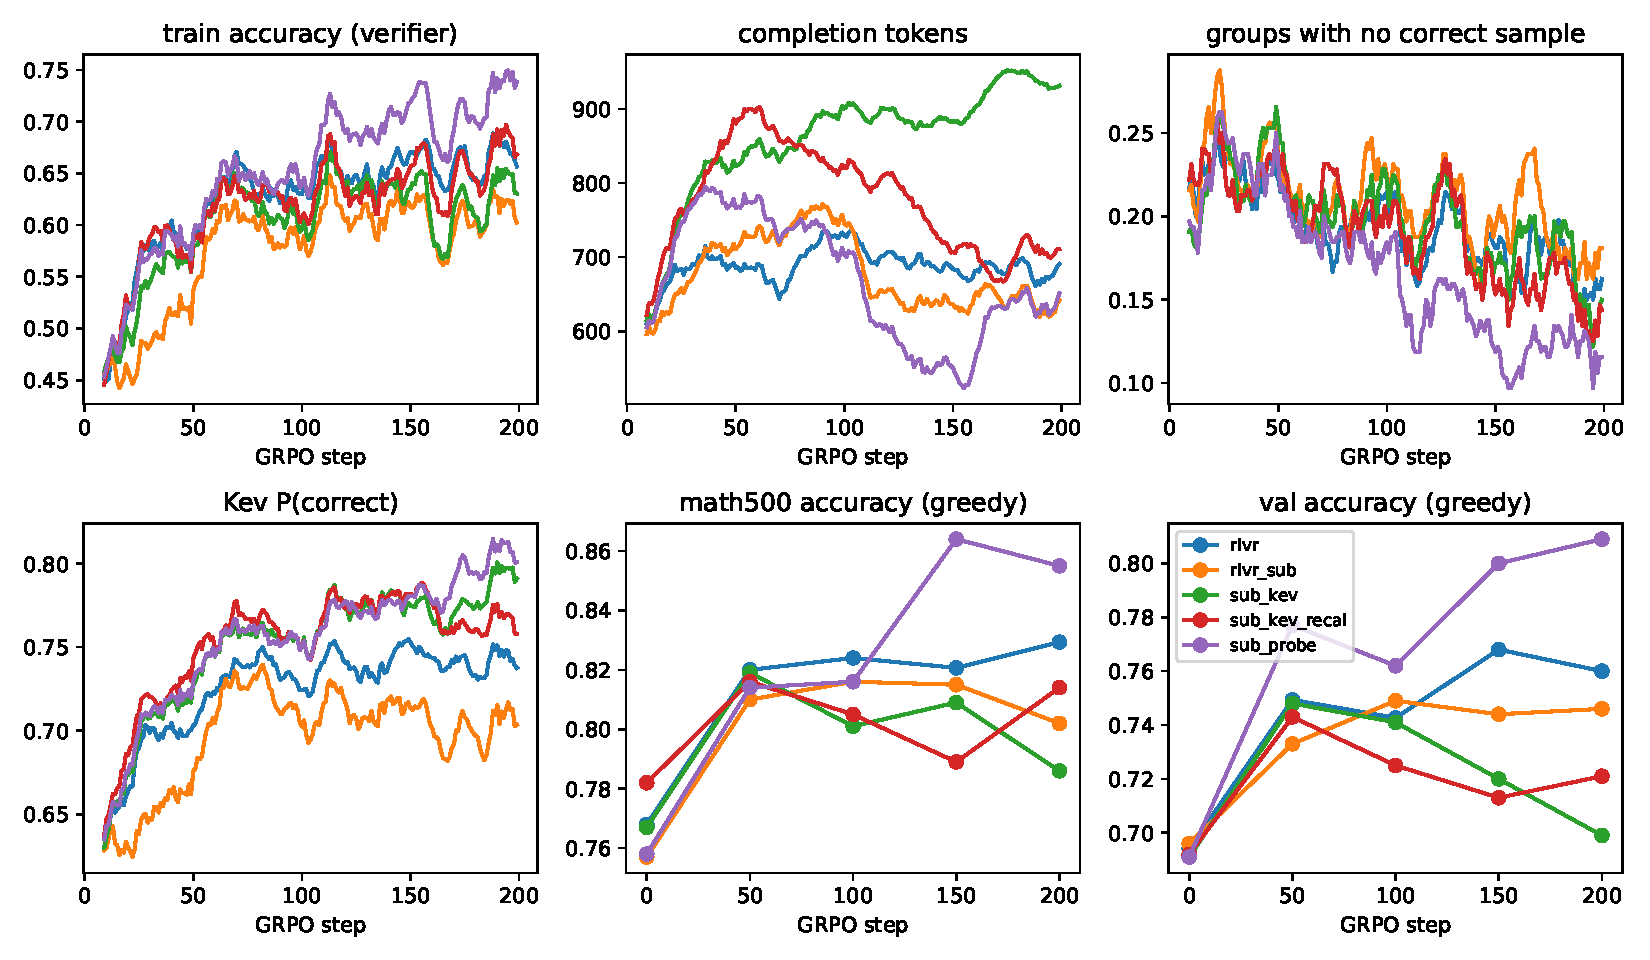
\includegraphics[width=\linewidth]{../../experiments/part3b_labels/results/training_curves.pdf}
\caption{Training curves (seed mean): verifier accuracy of all training completions (labelled or not), completion
tokens, share of groups with no correct completion and \kev{}'s $\pc$ on the training completions (10-step moving
averages), and greedy accuracy on MATH-500 and the validation set every 50 steps.}
\label{fig:sub-curves}
\end{figure}

\paragraph{Evaluation noise.} Across the \NUM{szruns_math500} runs in this comparison, the base model's MATH-500
accuracy at step 0 ranges from \NUM{szmin_math500}\% to \NUM{szmax_math500}\%, and a run's accuracy changes by
\NUM{lecabs_math500} points on average between its evaluations at steps 150 and 200. The final weights of each run are
evaluated twice on MATH-500, both times greedily: at step 200 with the periodic evaluations, and in the final
evaluation. The two results differ by \NUM{rptabs_math500} points on average and by up to \NUM{rptmax_math500}
(\NUM{rptruns_math500} runs).

\subsection{Does the judge pay for repetition?}\label{sec:res-repeat}

After the GRPO runs we tested whether \kev{} pays for what the policies of \texttt{sub\_kev} and
\texttt{sub\_kev\_recal} write after their first answer, with the probe of Part II (\file{dcjev/llm/repeat_probe.py};
Table~\ref{tab:repeat-probe}). \texttt{sub\_kev}'s policy restates its conclusion again and again;
\texttt{sub\_kev\_recal}'s solves the problem again in nearly the same words, like Part II's policies with \kev{} in
the reward. We cut the final MATH-500 solutions of seed 1 that repeat lines after their first answer, as if the policy
had stopped there. Solutions that repeat before their first answer, or whose first answer differs from their last,
were left out (\NUM{rpskip_subkev} and \NUM{rpskip_subrecal}). No edit changes the answer the verifier reads.

The part after the first answer raises the released \kev{}'s $\pc$, \texttt{sub\_kev}'s fill-in reward, by
\NUM{rpkevc_cutsubkev_1} \ci{\NUM{rpkevclo_cutsubkev_1}}{\NUM{rpkevchi_cutsubkev_1}} on right answers and by
\NUM{rpkevc_cutsubkev_0} \ci{\NUM{rpkevclo_cutsubkev_0}}{\NUM{rpkevchi_cutsubkev_0}} on wrong ones. On
\texttt{sub\_kev\_recal}'s solutions it raises it by \NUM{rpkevc_cutsubrecal_1}
\ci{\NUM{rpkevclo_cutsubrecal_1}}{\NUM{rpkevchi_cutsubrecal_1}} and \NUM{rpkevc_cutsubrecal_0}
\ci{\NUM{rpkevclo_cutsubrecal_0}}{\NUM{rpkevchi_cutsubrecal_0}}, for \NUM{rpkevcup_cutsubrecal_0} of the wrong ones.
Repetition as such is worth little: written into the base policy's solutions, it raises \kev{}'s $\pc$ by
\NUM{rpkevc_end3_1} on right answers and changes it by \NUM{rpkevc_end3_0} on wrong ones. So on the unlabelled
completions the fill-in reward paid for what these policies learned to write after their first answer, most of all on
wrong answers, to which the verifier would have given nothing. The probe scores with the released head. The head of
\texttt{sub\_kev\_recal} was refitted during training, and its own preference at the end of the run is not measured
here. The AR judge, which no condition used, rates \texttt{sub\_kev\_recal}'s solutions higher with the part after the
first answer (\NUM{rparc_cutsubrecal_1} on right answers) but \texttt{sub\_kev}'s endless restatements lower
(\NUM{rparc_cutsubkev_1} on right answers, \NUM{rparc_cutsubkev_0} on wrong ones).

\begin{table}[t]
\centering\small
\begin{tabular}{@{}lccccccc@{}}
\toprule
 & solutions & \multicolumn{2}{c}{\kev{} $\pc$} & \multicolumn{2}{c}{\kev{} $\pg$} & \multicolumn{2}{c}{AR $P_{\mathrm{a}}$} \\ \cmidrule(lr){3-4}\cmidrule(lr){5-6}\cmidrule(l){7-8}
 & right / wrong & right & wrong & right & wrong & right & wrong \\ \midrule
\multicolumn{8}{@{}l}{\emph{base policy's solutions, repetition added}} \\
\quad last two paragraphs twice more & 2436 / 1537 & $+$0.012 & $-$0.002 & $+$0.007 & $-$0.006 & $+$0.037 & $+$0.012 \\
\quad written twice & 2436 / 1564 & $+$0.012 & $-$0.003 & $+$0.006 & $-$0.004 & $+$0.029 & $+$0.007 \\
\multicolumn{8}{@{}l}{\emph{repeating final solutions of GRPO runs, as written against cut after the first answer}} \\
\quad \texttt{sub\_kev}, seed 1 & 351 / 66 & $+$0.031 & $+$0.049 & $+$0.016 & $+$0.031 & $-$0.018 & $-$0.074 \\
\quad \texttt{sub\_kev\_recal}, seed 1 & 318 / 81 & $+$0.059 & $+$0.110 & $+$0.030 & $+$0.095 & $+$0.034 & $+$0.034 \\
\bottomrule
\end{tabular}

\caption{What repetition is worth to the judges (the probe of Part II): P(with the repetition) minus P(without), on the
solutions the verifier accepts (right) and rejects (wrong), with the number of each. Top: the base policy's solutions
of Part II's judge study, with repetition added. Bottom: the final MATH-500 solutions of seed 1 that repeat lines, as
written against cut after their first answer. The released \kev{}'s $\pc$ and $\pg$ and the AR judge's
$P_{\mathrm{a}}$; intervals in the text resample problems.}
\label{tab:repeat-probe}
\end{table}

% Part III-B, discussion (included by main_en.tex).

\section{Discussion}\label{sec:discussion}

\paragraph{A good ranking is not enough.} The frozen \kev{} ranked the unlabelled completions well (AUROC
\NUM{fillauc_all_subkev}), and rewarding them with it still ended below dropping them. Two things it pays for beyond
correctness matter differently. Its generosity, a $\pc$ well above the share of correct completions, raises every
completion's expected reward by about the same amount and is removed by the group baseline. Its preference for
solutions that go on after their answer is not: such text leaves the verifier's label unchanged, so the labelled
completions never punish it, and the judge pays for it on the unlabelled ones (\S\ref{sec:res-repeat}). Both policies
of \texttt{sub\_kev} learned to repeat themselves. A fill-in reward has to be judged by what it pays for among
completions with the same verdict, which an AUROC for the verdict does not measure.

\paragraph{Recalibration fixes the numbers, not the preference.} Refitting the head on the labels so far made the
fill-in reward calibrated (ECE \NUM{fillece_all_subrecal} against \NUM{fillece_all_subkev}), and one of its two
policies still learned to repeat itself. A plausible reason, which these runs do not test directly: the refitted head
starts from the released one and is anchored to it, so it keeps the released head's preferences wherever the labels
say nothing, and repetition after the answer, which leaves the label unchanged, is such a place. A head trained from
scratch has no preference to keep, and neither of its policies repeated itself.

\paragraph{The probe's gain comes with a change of style.} \texttt{sub\_probe} ends \NUM{d_subprobe_math} points above
\texttt{rlvr\_sub} on MATH-500 and \NUM{d_subprobe_aime24} on AIME24, and above the full-label \texttt{rlvr} as well.
Both of its policies switched to drafting first, which no other run of this paper did; in this project's other GRPO
runs the same switch marks the best runs whatever their reward, \NUM{allveronlydraft} of them trained with the
verifier's reward alone (Part II, \S8.3). So with two seeds per condition we cannot say how much of the gain the probe is responsible for. If
the probe makes the switch more likely, which two of two runs suggest but cannot show, a scratch head trained on a
quarter of the labels would be a better fill-in reward than the judge it is built from, for a reason that has little
to do with how well it predicts the labels. More seeds of \texttt{sub\_probe} and \texttt{rlvr\_sub}, and runs that
force or forbid the draft opening, would tell.

\paragraph{Limitations.} One model (4B), one task, one label fraction (a quarter), 200 steps, two seeds per condition;
the recalibration's hyperparameters (anchor, buffer, steps) were set once and not tuned. The intervals resample
problems and not seeds. The style measures were defined after we had read the final completions. The repetition probe
scores with the released head, not with the refitted heads as they were at the end of training. Other experiments
shared the GPUs during training, so we report no training times.

\paragraph{Relation to the earlier versions.} Versions 1--3 of this paper reported a judge and a policy that improve
each other, long-horizon curves and anti-hacking results, none of which came from an experiment (see the notice at the
top and \file{CORRECTION.md}). This version runs a narrower setting that could be checked: partial labels, with only a
small head of the judge adapting. In it, adapting the judge's head fixed its calibration but not what it rewards, and
the best fill-in reward was a head trained from scratch, whose runs also changed how they write.


\section*{Reproducibility}
Code, prompts, raw logs (every GRPO step, with the fill-in rewards' agreement with the withheld labels, and every
evaluation) are in the repository (\texttt{experiments/part3b\_labels/}). The tables and every number in the text are
generated from them by \texttt{dcjev/analysis/part2.py} and \texttt{dcjev/analysis/paper\_numbers.py}.

\bibliographystyle{plainnat}
\bibliography{../common/refs}
\end{document}
